\documentclass{article}
\usepackage{tikz}
\usetikzlibrary{angles, quotes}
\usepackage{amssymb}
\usepackage{pgfplots}
\pgfplotsset{width=10cm,compat=1.9}
\usepgfplotslibrary{statistics}
\usepackage[left=2.54cm,right=2.54cm,top=2.54cm,bottom=2.54cm]{geometry}
\usepackage{tasks} %Paquete necesario para la producción de items horizontales para algunos ejercicios de tarea empleando el comando /begin{multicols}}{#}.../end{multicols} para ayudarnos a reducir las páginas
\usepackage{pdflscape} %comando que permite cambiar a orientación horizontal las hojas%
\usepackage{soul} %Paquete para permitir la compilación de acentos usando el comando {\hl{}}}\\
\sethlcolor{yellow(munsell)} %comando para definir el color para el subrayado usando el comando \hl
\usepackage[utf8]{inputenc}
\usepackage[spanish]{babel}
\usepackage{icomma}
\usepackage{ragged2e}		
\usepackage{siunitx}
\usepackage{url}
\usepackage[colorlinks=true, urlcolor=blue,  linkcolor=black, citecolor=green]{hyperref}
\usepackage{pdfpages}
\usepackage{blindtext} %Paquete que genera texto ficticio (dummy text) con el comando: \blindtext
\usepackage{cancel} %in the preamble gives you four different modes of striking through: \cancel{text to cancel} draws a diagonal line (slash) through its argument, \bcancel{text to cancel} uses the negative slope (a backslash), \xcancel{text to cancel} draws an X (actually \cancel plus \bcancel), \cancelto{〈value〉}{〈expression〉} draws a diagonal arrow through the 〈expression〉pointing to the 〈value〉 (math-mode only)
\usepackage{csquotes}
\usepackage{afterpage}
\usepackage{parskip} 
\usepackage{float}
\usepackage{enumitem}
%\usepackage{multicol}%Paquete que permite la creación aislada de columnas de texto. De esta forma se reduce la cantidad de páginas en nuestro documento
\usepackage{lipsum} %Paquete que genera texto de relleno al igual que \usepackage{blindtext}, se usa con el comando \lipsum[#-#] los #(hashtags) delimitan el número de páginas que deseamos ocupar del paquete lipsum para usarlos como relleno. 

% Definir el comando personalizado para la nota
\newcommand{\mynote}[1]{%
\begin{tikzpicture}[baseline=-0.75ex]
\node[draw, circle, fill=Apple Green!60, inner sep=2pt] (note) {\textbf{Nota:}};
\end{tikzpicture}%
\ \textit{#1}%
}

\newenvironment{Figura}
{\par\medskip\noindent\minipage{\linewidth}}
{\endminipage\par\medskip}
\usepackage{caption}
\usepackage[
backend=biber,
sorting=none,
url=true
]{biblatex} %bibliografía
\addbibresource{biblio.bib}
% Establecer el espacio entre las entradas de la bibliografía
\setlength{\bibitemsep}{1\baselineskip} % Puedes ajustar el valor según tus preferencias
\usepackage{amsmath,amsthm,amssymb,amsfonts}
\usepackage{pifont} %Permite la compilación del comando \xmark: es el símbolo de la tachita
\usepackage{mathtools} %permite la compilación de símbolos para matrices
\usepackage{empheq} %Paquete que se relaciona con \usepackage[most]{tcolorbox} para la creación de cuadros/cajas de colores para delimitar los resultados matemáticos o líneas de texto usando la línea de comando: \begin{empheq}[box={\mymath[colback=orange(webcolor)!70,drop lifted shadow]}]{equation*} \end{empheq}
\usepackage[most]{tcolorbox} %Paquete que se relaciona con \usepackage{empheq} para la creación de cuadros/cajas de colores para delimitar los resultados matemáticos o líneas de texto
\renewcommand{\qedsymbol}{$\blacksquare$}
\usetikzlibrary{positioning,decorations.pathreplacing} %Paquete que permite la compilación de llaves para cuadros sinópticos (brace diagram) 
\usepackage{schemata} %The schemata package is designed just for these brace diagrams
\usepackage{booktabs}

\newcommand\AB[2]{\schema{\schemabox{#1}}{\schemabox{#2}}} %comando o paquete necesario para crear cuadros sinópticos

\newtcbox{\mymath}[1][]{%
nobeforeafter, math upper, tcbox raise base,
enhanced, colframe=blue!30!black,
colback=blue!30, boxrule=1pt,
#1} %Comando importante para encasillar los resultados matemáticos en cajas de diferentes colores, se relaciona con los paquetes \usepackage{empheq} y \usepackage[most]{tcolorbox} 

\newenvironment{sysmatrix}[1]
{\left(\begin{array}{@{}#1@{}}}
{\end{array}\right)}
\newcommand{\ro}[1]{%
\xrightarrow{\mathmakebox[\rowidth]{#1}}%
}
\newlength{\rowidth}% row operation width
\AtBeginDocument{\setlength{\rowidth}{3em}}  %Comando importante para laproducción de lineas de operaciones entre matrices, método de Gauss o Gauss Jordan se relaciona con \newenvironment{sysmatrix}

%formato para cambiar el horario a español
\usepackage[spanish]{datetime2}
\DTMsetdatestyle{spanish}

\renewcommand{\today}{\DTMdisplaydate{\the\year}{\the\month}{\the\day }{-1}}
%%%%%%%%%%%%%%%%%%%%%%%%%%%%%%%%%%%%%%%%%

\usepackage{datetime}
\newcommand{\mycurrenttime}{\xxivtime}

%%%%%%%%%%%%%%%%%%%%%%%%%%%%%%%%%%%%%%%%%%%%%%%%%%%%%%%%%%%%%%%%%%%%%%%%%%%%%%%%%%%%%%%%%%%%%%%%%%%%%%%%%%%%%%%%%%%%%%%%%%%%%%%%%%%%%%%%%%%%%%%%%


%%%%%%%%%%%%%Caja de color para el título%%%%%%%%%%%%%%%%%%%%%%%%%%%%%%%%%%%%%%%%%%%%%%%%%%%%%%

\definecolor{myframecolor}{RGB}{1, 45, 75} % Prussian Blue
\definecolor{myboxcolor}{RGB}{0, 107, 92} % Apple Green

\newtcolorbox{mybox}{
enhanced,
colback=myboxcolor!7, % Color de fondo del cuadro
colframe=myframecolor, % Color del marco del cuadro
arc=0pt,
boxrule=1pt,
borderline west={2mm}{-10mm}{myframecolor}, % Borde en el lado izquierdo
sharp corners=southwest,
width=\linewidth,
before=\par\vspace{\bigskipamount}, % Espacio antes del cuadro
after=\par\vspace{\bigskipamount} % Espacio después del cuadro
}

%%%%%%%%%%%%%%%%%%%%%%%%%%%%%%%%%%%%%%%%%%%%%%%%%%%%%%%%%Nueva caja%%%%%%%%%%%%%%%%%%%%%%%%%%%%%%%%%%%%%%%%%%%%%%%%%%%%%%%%%%%%%%%%%

\newtcolorbox{mybox2}{
enhanced,
colback=Apple Green!7, % Color de fondo del cuadro
colframe=Apple Green, % Color del marco del cuadro
arc=0pt,
boxrule=1pt,
borderline west={2mm}{-10mm}{Apple Green}, % Borde en el lado izquierdo
sharp corners=southwest,
width=\linewidth,
before=\par\vspace{\bigskipamount}, % Espacio antes del cuadro
after=\par\vspace{\bigskipamount} % Espacio después del cuadro
}


\newcommand{\euler}{e} %Comando para producir letra e de euler
\newenvironment{remark}{\par\vfill\footnotesize % Vertical white space above the remark and smaller font size
\begin{list}{}{
	\leftmargin=80pt % Indentation on the left
	\rightmargin=60pt}\item\ignorespaces % Indentation on the right
\makebox[-2.5pt]{\begin{tikzpicture}[overlay]
		\node[draw=Horizon!60,line width=2.5pt,circle,fill=Horizon!25,font=\sffamily\bfseries,inner sep=4pt,outer sep=0pt] at (-19pt,5pt){\textcolor{Horizon}{Nota}};\end{tikzpicture}} % Blue Nota in a circle
\advance\baselineskip -1pt}{\end{list}\vskip5pt} % Tighter line spacing and white space after remark
\usepackage{graphicx}

\usepackage{titling}

\input{colores.tex}

%%Producir signos de cita textual``Asignatura''

\newcommand{\xmark}{\ding{55}} %%%comando que genera la tachita

\newenvironment{MyColorPar}[1]{%
\leavevmode\color{#1}\ignorespaces%
}{%
}%

%%%%%%%%%%%%%%%%%%% Título de la tarea, Nombre de alumno

\title{ \textcolor{Sun}{\textbf{Ejercicios}}}
\author{\emph{Tarea 2} $\boldsymbol{\mid}$ \textcolor{Tarawera}{\textbf{Principio de Hamilton}}}
\date{\today}

%%%%%%%%%%%%%%%%%%% Datos de la Materia

\usepackage{fancyhdr}
\fancypagestyle{plain}{%  the preset of fancyhdr 
\fancyhf{} % clear all header and footer fields
\fancyfoot[R]{
\includegraphics[width=2cm]{LogoFCFMBUAP (1).png}}
\fancyfoot[L]{{\bfseries{\thedate{}}} a las {\bfseries{\mycurrenttime{}}} horas{} (GMT-6, H. Puebla de Zaragoza, Pue)}
\fancyhead[L]{\textbf{Asignatura:} Mecánica Teórica}
\fancyhead[R]{\theauthor}
}
\makeatletter
\def\@maketitle{%
\newpage
\null%
\begin{center}%
\let \footnote \thanks
{\LARGE \@title \par}%
\vskip 1em%
%{\large \@date}%
\end{center}%
}
\makeatother

\usepackage{lipsum}  
\usepackage{cmbright}


%%%%%%%%%%%%%%%%%%%%%%%%%%%%%%%%%%%%%%%%%%%%%%%%%%%%%%%%%%%%%%%%%%%%%%%%%%%%%%%%%%%%%%%%%%%%%%%%%%%%%%%%%%%%%%%%%%%%%%%%%%%%%%%%%%%%%%%%%%%%%%%%%%%%%%%%%%%%%%%%%%%%%%%%%%%%%%%%%%%%%%%%%%%%%%%%%%%%%%

\begin{document}



\maketitle

%%%%%%%%%%%%%%%%%%% Datos del profesor, campus, aula e integrantes

\begin{mybox2}
\noindent
\begin{tabular}{@{}p{3.7cm}p{10.4cm}@{}}
\textbf{Profesor} & Dr. Gilberto Silva Ortigoza \\[3pt]
\textbf{Campus / Facultad} & \textcolor{prussianblue}{\textbf{C.U. BUAP}} / \textcolor{trueblue}{\textbf{FCFM}} \\[3pt]
\textbf{Edificio / Salón} & \textcolor{prussianblue}{\textbf{EMA4}} / \textcolor{trueblue}{\textbf{302}} \\[6pt]
\textbf{Integrantes} &
\begin{minipage}[t]{\linewidth}
\raggedright
\textbf{González-Salud}, S.\textsuperscript{1};\,
\textbf{Victoria-García}, A. A.\textsuperscript{2};\,
\textbf{Cruz-Toledo}, F. A.\textsuperscript{3};\,
\textbf{Calderón-Muñoz}, J. C.\textsuperscript{(oyente)4};\,
\textbf{Gómez-González}, F. S.\textsuperscript{5};\,
\textbf{Hernández-Mejía}, M. I.\textsuperscript{6};\,
\textbf{Torres-Luna}, N. A.\textsuperscript{7};\,
\textbf{Martínez-Solorio}, R. J.\textsuperscript{8};\,
\textbf{Arroyo-Gonzalez}, D.\textsuperscript{9};\,
\textbf{Sandoval-Zonotl}, H.\textsuperscript{10};\,
\textbf{Peralta-Rebolledo}, A.\textsuperscript{11};\,
\textbf{Gómez-Alatorre}, A. D.\textsuperscript{12};\,
\textbf{Ballinas-García}, J. A.\textsuperscript{13}
\end{minipage}
\end{tabular}
\end{mybox2}
\vspace{1cm}




\section*{\textcolor{Tarawera}{\textbf{Lista de problemas}}}
\addcontentsline{toc}{section}{\textcolor{Tarawera}{\textbf{Problemas: cap 2}}}

\setlength{\columnsep}{2cm}
%\begin{multicols}{2}

\begin{enumerate}[label={{\textcolor{trueblue}{\textbf{Pr.} \arabic*.1}}}, start=2]
  \item \textbf{Problema 1} Hacer un gráfico del espacio de configuraciones para el péndulo esférico. Justifique su respuesta.
\end{enumerate}

\textcolor{Cinnabar}{\textbf{Soluci\'on:}}

Un \textbf{péndulo esférico} consiste en una masa $m$ sujeta a un punto fijo
mediante una varilla rígida de longitud $l$.  
A diferencia del péndulo plano, que sólo oscila en un mismo plano,
aquí la masa puede moverse en cualquier dirección alrededor del punto
de suspensión.  

\begin{figure}[H] % usa [htbp] si no quieres fijar posición estricta
  \centering
  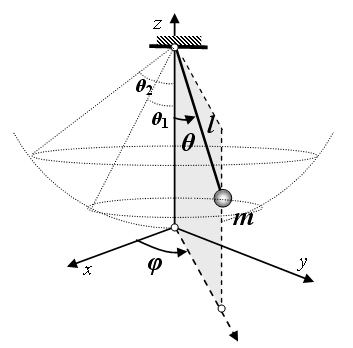
\includegraphics[width=0.42\textwidth]{pendulo_esferico.jpg} % o figuras/pendulo_esferico.jpg
  \caption{Esquema del péndulo esférico: la masa $m$ unida por una varilla de longitud $l$ y los ángulos $\theta$ y $\phi$.}
  \label{fig:pendulo-esferico}
\end{figure}

Como la varilla no se alarga ni se acorta, la distancia entre el punto fijo
y la masa permanece constante, de modo que la bolita recorre siempre
la superficie de una esfera de radio $l$.

\vspace{0.3cm}
\noindent\textbf{Vector de posición.}  
La posición de la masa se describe mediante el vector
\begin{equation}
\begin{split}
\mathbf r &= x\,\hat x + y\,\hat y + z\,\hat z 
\end{split}\label{eq:vector-posicion}
\end{equation}
Dado que el movimiento ocurre sobre una esfera, es práctico usar
\textbf{coordenadas esféricas} $(r,\theta,\phi)$

La relación entre estas coordenadas y las cartesianas es
\begin{equation}
\begin{split}
x &= r \sin\theta \cos\phi,\\
y &= r \sin\theta \sin\phi,\\
z &= r \cos\theta 
\end{split}\label{eq:rel-cart-esf}
\end{equation}

Como $r=l$ es constante,
\begin{equation}
\begin{split}
\mathbf r(l,\theta,\phi)
&= \bigl(l\sin\theta\cos\phi,\;
          l\sin\theta\sin\phi,\;
          l\cos\theta\bigr)
\end{split}\label{eq:r-l-theta-phi}
\end{equation}
Cada par de ángulos $(\theta,\phi)$ identifica un punto específico de la
superficie de la esfera y, por lo tanto, una orientación particular de la varilla

\vspace{0.3cm}
\noindent\textbf{Espacio de configuraciones.}  
El \emph{espacio de configuraciones} es el conjunto
de todas las posiciones que la masa puede ocupar.  
Aquí son todos los puntos de una esfera de radio $l$, ya que la
única condición es que la distancia al origen sea constante:
\begin{equation}
\begin{split}
|\mathbf r| &= l .
\end{split}\label{eq:constraint-r-constante}
\end{equation}
Así, el espacio de configuraciones coincide con la superficie esférica de radio $l$

\vspace{0.35cm}
\noindent\textbf{¿Qué es \( Q = S^{2} \)?}  
\begin{itemize}
  \item \(Q\) representa todas las configuraciones posibles del sistema.
  \item \(S^{2}\) es la \emph{superficie} de una esfera (no su volumen).
  \item Decir \(Q = S^{2}\) significa que cada orientación de la varilla corresponde a un punto único en esa superficie.
\end{itemize}
Se necesitan dos números (\(\theta,\phi\)) para describir cada configuración, como latitud y longitud en un globo.

\begin{figure}[H] 
  \centering
  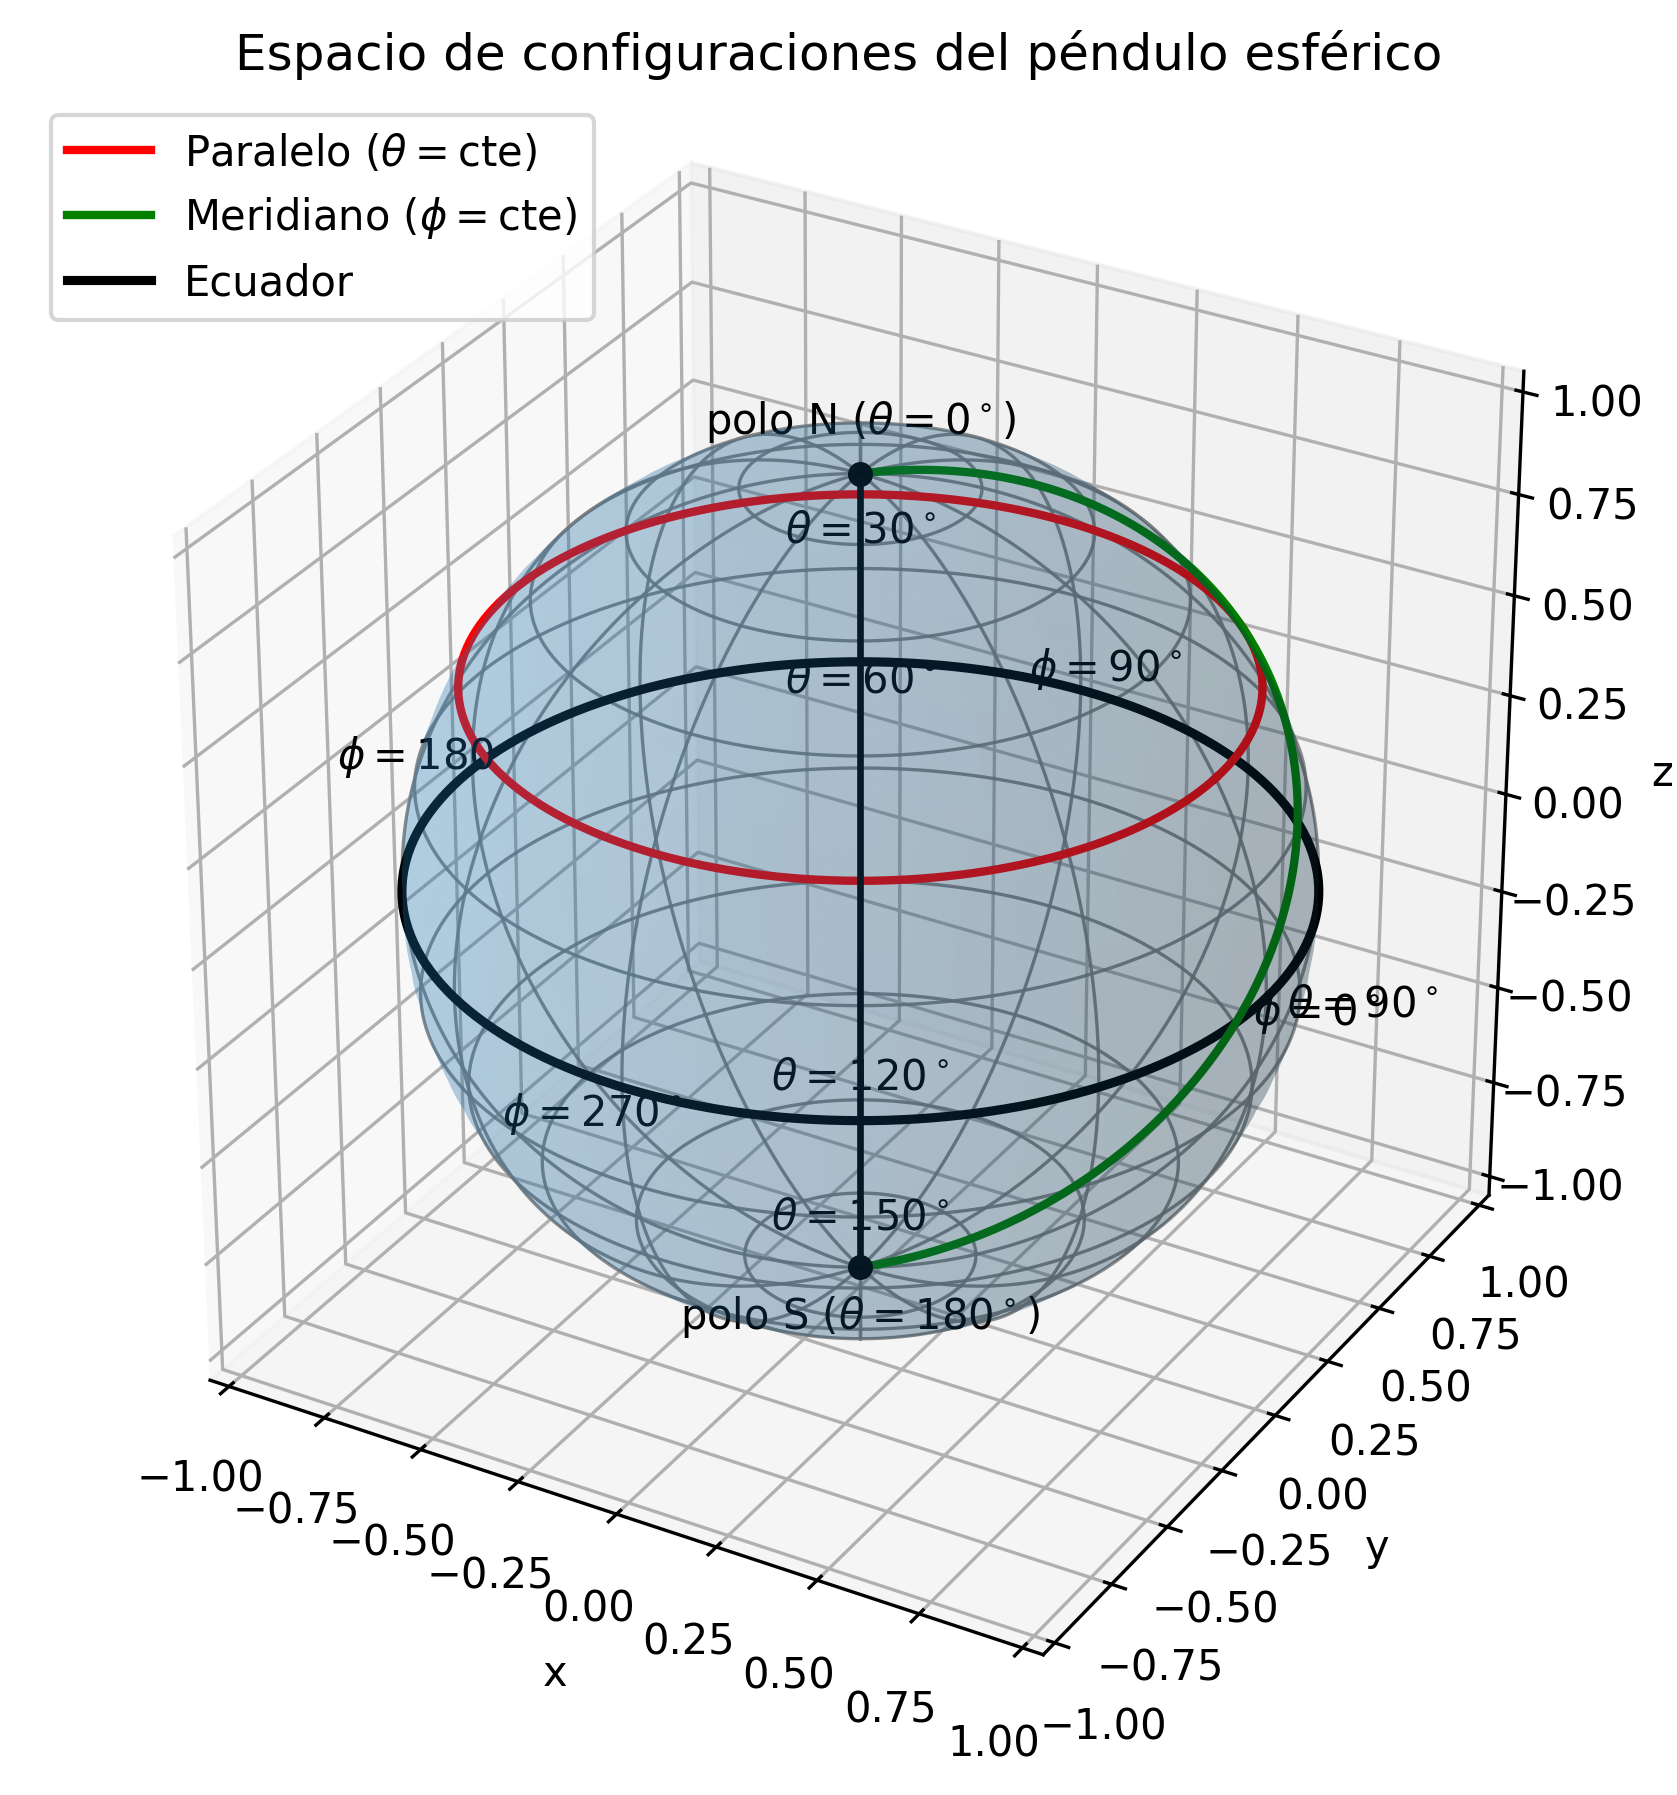
\includegraphics[width=0.62\textwidth]{pendulo_S.png}
 \caption{Espacio de configuraciones del péndulo esférico $Q$: cada punto de la superficie esférica representa una orientación posible de la varilla de longitud $l$, parametrizada por los ángulos $\theta$ (inclinación) y $\phi$ (azimutal).}
  \label{fig:pendulo-esferico}
\end{figure}

\subsection*{Parámetros del espacio de configuraciones}
\begin{itemize}
    \item $l$ es el radio de la esfera, es decir, la distancia desde el centro hasta cualquier punto de su superficie.
    \item El ángulo $\theta$ (polar) mide la inclinación del vector $\mathbf{r}$ con respecto al eje $z$.
    \item El ángulo $\phi$ (azimutal) mide la rotación del vector $\mathbf{r}$ alrededor del eje $z$ en el plano $xy$.
\end{itemize}

\subsection*{Curvas con $\theta$ constante: paralelos}
\begin{itemize}
    \item Mantener $\theta$ fijo y variar $\phi$ describe un \textbf{paralelo}, una circunferencia horizontal en la superficie de la esfera.
    \item En la figura se resalta en \textcolor{red}{rojo} el paralelo correspondiente a $\theta=60^\circ$ y en \textcolor{black}{negro} el ecuador para $\theta=90^\circ$.
\end{itemize}

\subsection*{Curvas con $\phi$ constante: meridianos}
\begin{itemize}
    \item Mantener $\phi$ fijo y variar $\theta$ describe un \textbf{meridiano}, una circunferencia vertical que pasa por los polos.
    \item En la figura se muestra en \textcolor{green!70!black}{verde} el meridiano correspondiente a $\phi=45^\circ$.
\end{itemize}

Como se aprecia, la esfera está recubierta por una red de meridianos y paralelos.  
Cada punto de esta superficie representa una posible configuración del péndulo esférico y queda determinado únicamente por los dos ángulos $(\theta,\phi)$.



\vspace{0.4cm}
\noindent\textbf{Restricciones y grados de libertad.}
\begin{enumerate}
  \item \textbf{Longitud fija:}
  \begin{equation}
  \begin{split}
  f_1(x,y,z) &= x^{2}+y^{2}+z^{2}-l^{2} = 0 
  \end{split}\label{eq:constraint-longitud}
  \end{equation}

  \item \textbf{En coordenadas esféricas:}
  \begin{equation}
  \begin{split}
  x&=l\sin\theta\cos\phi,\qquad
  y=l\sin\theta\sin\phi,\qquad
  z=l\cos\theta
  \end{split}\label{eq:coordenadas-esfericas-fijas}
  \end{equation}

  \item \textbf{¿Hay más constricciones o ligaduras?:}  
        No hay contacto con superficies ni restricciones adicionales.
\end{enumerate}

Entonces partimos de tres coordenadas cartesianas y tenemos una restricción holónoma, por lo que los
\textbf{grados de libertad} son
\begin{equation}
\begin{split}
n &= 3 - 1 = 2 ,
\end{split}\label{eq:grados-libertad}
\end{equation}
coincidiendo con las dos coordenadas independientes $\theta$ y $\phi$.

\vspace{0.4cm}
\noindent\textbf{Lagrangiana y ecuaciones de movimiento}

Para describir la dinámica de este \textbf{péndulo esférico} usamos el formalismo lagrangiano.  
La \underline{energía cinética} de la masa es
\begin{equation}
\begin{split}
T &= \frac{1}{2}m v^{2}
\end{split}\label{eq:def-T}
\end{equation}

\noindent\textbf{Velocidad}

Partimos de
\begin{equation}
\begin{split}
\mathbf r(t)
&= r(t)\bigl(\sin\theta(t)\cos\phi(t),\;
             \sin\theta(t)\sin\phi(t),\;
             \cos\theta(t)\bigr)
\end{split}\label{eq:r-general}
\end{equation}
Derivando componente a componente (regla del producto) y luego imponiendo $r=l$ y $\dot r=0$:
\begin{equation}
\begin{split}
\dot x &= \dot r\sin\theta\cos\phi
         + r\dot\theta\cos\theta\cos\phi
         - r\dot\phi\sin\theta\sin\phi,\\
\dot y &= \dot r\sin\theta\sin\phi
         + r\dot\theta\cos\theta\sin\phi
         + r\dot\phi\sin\theta\cos\phi,\\
\dot z &= \dot r\cos\theta
         - r\dot\theta\sin\theta 
\end{split}\label{eq:componentes-derivadas}
\end{equation}
Con $r=l$ y $\dot r=0$:
\begin{equation}
\begin{split}
\dot{\mathbf r}
&= \bigl(
l\dot\theta\cos\theta\cos\phi - l\dot\phi\sin\theta\sin\phi,\;
l\dot\theta\cos\theta\sin\phi + l\dot\phi\sin\theta\cos\phi,\;
-\,l\dot\theta\sin\theta
\bigr)
\end{split}\label{eq:r-punto}
\end{equation}

Cuadrados de las componentes:
\begin{equation}
\begin{split}
\dot x^2
&= l^2\!\left(\dot\theta\cos\theta\cos\phi - \dot\phi\sin\theta\sin\phi\right)^2\\
&= l^2\!\left(
\dot\theta^2\cos^2\theta\cos^2\phi
-2\dot\theta\dot\phi\,\cos\theta\sin\theta\cos\phi\sin\phi
+\dot\phi^2\sin^2\theta\sin^2\phi
\right),
\end{split}\label{eq:xdot2}
\end{equation}
\begin{equation}
\begin{split}
\dot y^2
&= l^2\!\left(\dot\theta\cos\theta\sin\phi + \dot\phi\sin\theta\cos\phi\right)^2\\
&= l^2\!\left(
\dot\theta^2\cos^2\theta\sin^2\phi
+2\dot\theta\dot\phi\,\cos\theta\sin\theta\sin\phi\cos\phi
+\dot\phi^2\sin^2\theta\cos^2\phi
\right),
\end{split}\label{eq:ydot2}
\end{equation}
\begin{equation}
\begin{split}
\dot z^2
&= l^2\,\dot\theta^2\sin^2\theta 
\end{split}\label{eq:zdot2}
\end{equation}

Tenemos: 
\begin{equation}
\begin{split}
\dot x^2+\dot y^2
&= l^2\Big[
\dot\theta^2\cos^2\theta(\cos^2\phi+\sin^2\phi)
+\dot\phi^2\sin^2\theta(\sin^2\phi+\cos^2\phi)\\
&\quad -\,2\dot\theta\dot\phi\,\cos\theta\sin\theta\cos\phi\sin\phi
+2\dot\theta\dot\phi\,\cos\theta\sin\theta\sin\phi\cos\phi
\Big] \\
&= l^2\left(\dot\theta^2\cos^2\theta+\dot\phi^2\sin^2\theta\right).
\end{split}\label{eq:suma-xy}
\end{equation}

Rapidez:
\begin{equation}
\begin{split}
v^2
&= \dot x^2+\dot y^2+\dot z^2 \\
&= l^2\left(\dot\theta^2\cos^2\theta+\dot\phi^2\sin^2\theta\right)
  + l^2\,\dot\theta^2\sin^2\theta \\
&= l^2\left[\dot\theta^2(\cos^2\theta+\sin^2\theta)
            + \sin^2\theta\,\dot\phi^2\right] \\
&= l^{2}\bigl(\dot\theta^{2}+\sin^{2}\theta\,\dot\phi^{2}\bigr)
\end{split}\label{eq:v2}
\end{equation}

Por lo tanto, la energía cinética es
\begin{equation}
\begin{split}
T
&= \frac{1}{2} m v^{2}
  = \frac{1}{2} m l^{2}\!
      \left(\dot{\theta}^{2}
            + \sin^{2}\theta\,\dot{\phi}^{2}\right)
\end{split}\label{eq:T}
\end{equation}

El potencial gravitatorio (referencia $V=0$ en el plano por el punto de suspensión) es
\begin{equation}
\begin{split}
U &= m g z = m g l \cos\theta 
\end{split}\label{eq:U}
\end{equation}

La \textbf{Lagrangiana} $L=T-U$ resulta en:
\begin{equation}
\begin{split}
L
&= \frac{1}{2} m l^2 \left(\dot\theta^2 + \sin^2\theta\,\dot\phi^2 \right)
   - m g l \cos\theta 
\end{split}\label{eq:L}
\end{equation}

Ecuaciones de Euler–Lagrange para $q_i\in\{\theta,\phi\}$:
\begin{equation}
\begin{split}
\frac{d}{dt}\!\left(\frac{\partial L}{\partial \dot q_i}\right)
-\frac{\partial L}{\partial q_i} &= 0 
\end{split}\label{eq:EL-general}
\end{equation}

Para $\theta$:
\begin{equation}
\begin{split}
\frac{\partial L}{\partial \dot\theta} &= m l^{2}\dot{\theta},\\
\frac{\partial L}{\partial \theta}
&= m l^{2}\sin\theta\cos\theta\,\dot\phi^{2}
 + m g l \sin\theta,
\end{split}\label{eq:parciales-theta}
\end{equation}
y por \eqref{eq:EL-general} resulta
\begin{equation}
\begin{split}
\ddot\theta
 - \sin\theta\cos\theta\,\dot\phi^{2}
 + \frac{g}{l}\sin\theta &= 0 
\end{split}\label{eq:ecuacion-theta}
\end{equation}

Para $\phi$:
\begin{equation}
\begin{split}
\frac{\partial L}{\partial \dot\phi} &= m l^{2}\sin^{2}\theta\,\dot\phi,\\
\frac{\partial L}{\partial \phi} &= 0,
\end{split}\label{eq:parciales-phi}
\end{equation}
de donde
\begin{equation}
\begin{split}
\frac{d}{dt}\!\left(m l^{2}\sin^{2}\theta\,\dot\phi\right) &= 0 
\end{split}\label{eq:ecuacion-phi}
\end{equation}
La cantidad conservada es el momento conjugado
\begin{equation}
\begin{split}
p_\phi &= m l^{2}\sin^{2}\theta\,\dot\phi ,
\end{split}\label{eq:pphi}
\end{equation}
que corresponde al \emph{momento angular alrededor del eje $z$}

De \eqref{eq:L} se observa que $L$ no depende de forma explícita de $\phi$; por lo tanto, $\phi$ es
\emph{coordenada cíclica} y su momento conjugado \eqref{eq:pphi} se mantiene constante.
Esta simetría de rotación alrededor del eje $z$ significa que todas las
orientaciones con el mismo valor de $\theta$ son equivalentes salvo por un giro,
pues no hay ningún torque externo en esa dirección.

La única restricción geométrica es \eqref{eq:constraint-r-constante}, es decir,
el extremo de la varilla siempre debe cumplir $|\mathbf r| = l$.
En consecuencia, las configuraciones posibles del sistema corresponden
exactamente a los puntos de la \emph{superficie de una esfera} de radio $l$,
determinados únicamente por los dos ángulos independientes $(\theta,\phi)$.
Por ello, el “gráfico del espacio de configuraciones” solicitado en el problema
es una esfera de radio $l$, donde cada punto representa una orientación de la
varilla descrita por el par de ángulos $(\theta,\phi)$. En la figura se muestra
esa esfera con meridianos y paralelos para resaltar esta parametrización.


\vspace{0.5cm}
\begin{center}
\begin{tikzpicture}
	% Dibuja círculos rellenos en diferentes colores
	\fill[bittersweet] (0,0) circle (0.17cm);
	\fill[Apple Green] (0.6,0) circle (0.17cm);
	\fill[trueblue] (1.2,0) circle (0.17cm);
	\fill[Aguamarina] (1.8,0) circle (0.17cm);
	\fill[Sun] (2.4,0) circle (0.17cm);
	\fill[orange(colorwheel)] (3.0,0) circle (0.17cm);
	\fill[Pesto] (3.6,0) circle (0.17cm);
	\fill[blue-violet] (4.2,0) circle (0.17cm);
	\fill[ticklemepink] (4.8,0) circle (0.17cm);
	\fill[Gallery] (5.4,0) circle (0.17cm);
	\fill[Mantle] (6.0,0) circle (0.17cm);
	\fill[Nevada] (6.6,0) circle (0.17cm);
	\fill[onyx] (7.2,0) circle (0.17cm);
	% Agrega más círculos o modifica los colores según sea necesario
\end{tikzpicture}
\end{center}  \vspace{0.5cm}


\begin{enumerate}[label={{\textcolor{trueblue}{\textbf{Pr.} \arabic*.2}}}, start=2]
  \item \textbf{Problema 2} Una representación paramétrica del toro está dada por
  \[
    x=(l_1+l_2\cos\phi_2)\cos\phi_1,\quad
    y=(l_1+l_2\cos\phi_2)\sin\phi_1,\quad
  \]
  \[ z=l_2\sin\phi_2, \]
  
  
donde $l_{1}$ y $ l_{2}$ son constantes tales que $l_{1}$ $>$ $l_{2}$, $0\leq \phi_{1}\leq 2\pi$ y $0 \leq  \phi_{2}\leq 2\pi$. Hacer el gráfico para el caso especial $l_{1} =1$ y $l_{2}=0\text{.}5$. Además, en diferente color incluya las circunferencias dadas por ($\phi=0$, $\pi$, $0\leq \phi_{2}\leq 2\pi$) y ($0\leq \phi_{1}\leq 2\pi, \phi_{2}=0, \pi$) 
\end{enumerate}

\textcolor{Cinnabar}{\textbf{Soluci\'on:}}

Las ecuaciones paramétricas para el toro son:
\begin{align*}
    x &= (l_1 + l_2\cos\phi_2)\cos\phi_1 \\
    y &= (l_1 + l_2\cos\phi_2)\sin\phi_1 \\
    z &= l_2\sin\phi_2
\end{align*}
Donde se especifican las constantes $l_1=1$ y $l_2=0.5$, y los rangos angulares $0 \le \phi_1 \le 2\pi$ y $0 \le \phi_2 \le 2\pi$.

\subsection*{Parámetros:}
\begin{itemize}
    \item $l_1$ es el radio mayor, la distancia desde el centro del toro hasta el centro del "tubo".
    \item $l_2$ es el radio menor, que corresponde al radio de la sección transversal circular del "tubo".
    \item El ángulo $\phi_1$ representa la rotación alrededor del eje z, barriendo el círculo mayor del toro (movimiento toroidal).
    \item El ángulo $\phi_2$ representa la rotación alrededor del círculo que forma el "tubo" (movimiento poloidal).
\end{itemize}



Las circunferencias solicitadas se muestran en \textbf{rojo} y \textbf{verde} sobre la superficie del toro y corresponden a fijar el valor de uno de los ángulos mientras el otro varía en todo su rango.

\subsection*{Circunferencias con $\phi_1$ constante ($\phi_1=0, \pi$):}
\begin{itemize}
    \item Cuando $\phi_1$ es constante, nos movemos a lo largo de la sección transversal del "tubo" del toro.
    \item Para $\phi_1=0$, la circunferencia se encuentra en el plano x-z (con $y=0$).
    \item Para $\phi_1=\pi$, la circunferencia también está en el plano x-z pero en el lado opuesto del toro.
    \item Estas dos curvas son las circunferencias poloidales (verticales) del toro.
\end{itemize}

\subsection*{Circunferencias con $\phi_2$ constante ($\phi_2=0, \pi$):}
\begin{itemize}
    \item Cuando $\phi_2$ es constante, nos movemos a lo largo del toro en una trayectoria paralela al plano xy.
    \item Para $\phi_2=0$, $\cos(\phi_2)=1$ y $z=0$. Esto traza la circunferencia exterior del toro, con un radio de $l_1+l_2=1.5$.
    \item Para $\phi_2=\pi$, $\cos(\phi_2)=-1$ y $z=0$. Esto traza la circunferencia interior del toro (el "agujero"), con un radio de $l_1-l_2=0.5$.
    \item Estas dos curvas son las circunferencias toroidales (horizontales) del toro.
\end{itemize}

Como se puede observar en la Figura~\ref{fig:toro}, se destacan las circunferencias toroidales y poloidales.


\begin{figure}[h!] 
    \centering 
    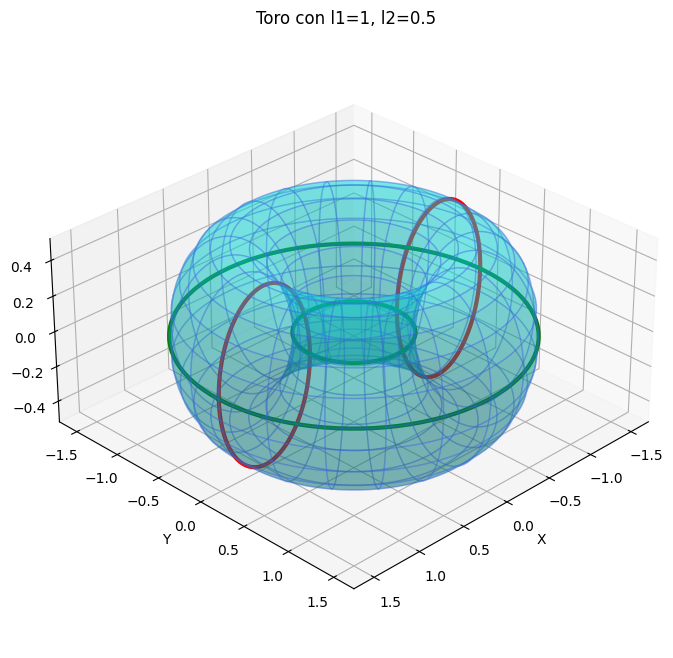
\includegraphics[width=0.8\textwidth]{toro.png} 
    \caption{Toro generado con los parámetros $l_{1}=1$ y $l_{2}=0.5$.} 
    \label{fig:toro} 
\end{figure}

\vspace{0.5cm}
\begin{center}
\begin{tikzpicture}
	% Dibuja círculos rellenos en diferentes colores
	\fill[bittersweet] (0,0) circle (0.17cm);
	\fill[Apple Green] (0.6,0) circle (0.17cm);
	\fill[trueblue] (1.2,0) circle (0.17cm);
	\fill[Aguamarina] (1.8,0) circle (0.17cm);
	\fill[Sun] (2.4,0) circle (0.17cm);
	\fill[orange(colorwheel)] (3.0,0) circle (0.17cm);
	\fill[Pesto] (3.6,0) circle (0.17cm);
	\fill[blue-violet] (4.2,0) circle (0.17cm);
	\fill[ticklemepink] (4.8,0) circle (0.17cm);
	\fill[Gallery] (5.4,0) circle (0.17cm);
	\fill[Mantle] (6.0,0) circle (0.17cm);
	\fill[Nevada] (6.6,0) circle (0.17cm);
	\fill[onyx] (7.2,0) circle (0.17cm);
	% Agrega más círculos o modifica los colores según sea necesario
\end{tikzpicture}
\end{center}  \vspace{0.5cm}


\begin{enumerate}[label={{\textcolor{trueblue}{\textbf{Pr.} \arabic*.3}}}, start=2]

  \item \textbf{Problema 3} Usar las ecuaciones
  \begin{align}
    \mathbf r_1(\phi_1,\phi_2)&=l_1(\sin\phi_1\,\hat y-\cos\phi_1\,\hat z)\\
    \mathbf r_2(\phi_1,\phi_2)&=(l_1\sin\phi_1+l_2\sin\phi_2)\hat y-(l_1\cos\phi_1+l_2\cos\phi_2)\hat z
  \end{align}
  para obtener el Lagrangiano del péndulo doble plano. Ahora suponga que $\phi_{1} \approx 0$ y $\phi_{2}\approx 0$, desarrolle en serie de potencias las funciones trigonométricas que aparecen en el Lagrangiano y obtenga una aproximación del Lagrangiano a segundo orden en $\phi_{1}$, $\phi_{2}$, $\dot{\phi}_{1}$ y $\dot{\phi}_{2}$. Finalmente, obtenga las ecuaciones de Lagrange del Lagrangiano aproximado.
\end{enumerate}

\textcolor{Cinnabar}{\textbf{Soluci\'on:}} Dados los vectores de posici\'on $\mathbf{r}_i$ podemos determinar el Lagrangiano inmediatamente; n\'otese
\begin{equation}
    L=\sum_{i=1}^{2}\bigl(T-U\bigr)=\sum_{i=1}^{2}\left(\frac{1}{2}m_i\mathbf{\dot{r}}_i^2+m_i\mathbf{r}_i\cdot\mathbf{g}\right),
\end{equation}
donde la suma es para cada part\'icula y hemos tomado $U_i=-m_i\mathbf{r}_i\cdot\mathbf{g}$. Ahora bien, hemos de ser cuidadosos cuando elijamos nuestro sistema coordenados (no es lo mismo $\mathbf{g}=-g\,\mathbf{\hat{y}}$ que $\mathbf{g}=-g\,\mathbf{\hat{z}}$); para ello, hemos de analizar los vectores posici\'on. Primero que nada (ser\'a \'util de aqu\'i en adelante), observemos
\begin{align}
    \mathbf{\dot{r}}_1&=l_1\dot{\phi}_1(\cos\phi_1\,\mathbf{\hat{y}}+\sin\phi_1\,\mathbf{\hat{z}}), \\
    \mathbf{\dot{r}}_2&=(l_1\dot{\phi}_1\cos\phi_1+l_2\dot{\phi}_2\cos\phi_2)\,\mathbf{\hat{y}}+(l_1\dot{\phi}_1\sin\phi_1+l_2\dot{\phi}_2\sin\phi_2)\,\mathbf{\hat{z}}.
\end{align}
Consideremos entonces $m_2=0$, de forma que tengamos un \'unico p\'endulo en $\mathbf{r}_1$ cuyas ecuaciones conocemos y podamos comparar; as\'i
\begin{equation*}
    T_1 =\frac{1}{2}m_1\mathbf{\dot{r}}_1\cdot\mathbf{\dot{r}}_1
    =\frac{1}{2}m_1l_1^2\dot{\phi}^2_1\left(\cos^2\phi+\sin^2\phi\right)
    =\frac{1}{2}m_1l_1^2\dot{\phi}^2_1,
\end{equation*}
\begin{equation*}
    L_1=T_1-U_1=\frac{1}{2}m_1 l_1^2 \dot{\phi}^2_1+m_1\mathbf{r}_1\cdot\mathbf{g},
\end{equation*}
y entonces
\begin{align*}
    -\frac{\partial L}{\partial \phi_1}+\frac{\mathrm{d}}{\mathrm{d}t}\left(\frac{\partial L}{\partial \phi_1}\right)
    =-\left(m_1\frac{\partial \mathbf{r}_1}{\partial\phi_1}\cdot\mathbf{g}\right)+\frac{\mathrm{d}}{\mathrm{d}t}\left(m_1 l_1^2 \dot{\phi}_1\right)
    =-m_1\frac{\partial\mathbf{r}_1}{\partial\phi_1}\cdot\mathbf{g}+m_1l_1^2\ddot{\phi}_1
    \overset{!}=m_1l_1^2\left(\ddot{\phi}_1+\frac{g}{l_1}\sin\phi_1\right)
    \overset{!}=0,
\end{align*}
donde en la pen\'ultima igualdad igualamos a lo que se espera naturalmente de un p\'endulo; de esta forma, observamos que ha de cumplirse
\begin{equation}
    g_1l_1\sin\phi_1=\frac{\partial \mathbf{r}_1}{\partial \phi_1}\cdot\mathbf{g}=l_1(\cos\phi_1\;\mathbf{\hat{y}}+\sin\phi_1\,\mathbf{z})\cdot\mathbf{g},
\end{equation}
y dado que esto debe cumplirse para todo $\phi_1$, no queda de otra sino que $\mathbf{g}=-g\,\mathbf{\hat{z}}$. Ahora que ya conocemos nuestro $\mathbf{g}$, podemos conocer el lagrangiano expl\'icitamente y a partir de este obtenemos las ecuaciones de movimiento. Tenemos
\begin{align}
    T_2&=\frac{1}{2}m_2\mathbf{\dot{r}}_2^2=\frac{1}{2}m_2\left[(l_1\dot{\phi}_1\cos\phi_1+l_2\dot{\phi}_2\cos\phi_2)^2+(l_1\dot{\phi}_1\sin\phi_1+l_2\dot{\phi}_2\sin\phi_2)^2\right] \nonumber \\
    &=\frac{1}{2}m_2\left[(l_1^2\dot{\phi}^2_1\cos^2\phi_1 + l_2^2\dot{\phi}^2_2\cos^2\phi_2 + 2l_1l_2\dot{\phi}_1\dot{\phi}_2\cos\phi_1\cos\phi_2) + (l_1^2\dot{\phi}^2_1\sin^2\phi_1 + l_2^2\dot{\phi}^2_2\sin^2\phi_2 + 2l_1l_2\dot{\phi}_1\dot{\phi}_2\sin\phi_1\sin\phi_2)\right] \nonumber \\
    &=\frac{1}{2}m_2\left(l_1^2\dot{\phi}^2_1+l_2^2\dot{\phi}^2_2+2l_1l_2\dot{\phi}_1\dot{\phi}_2\cos(\phi_1-\phi_2)\right),
\end{align}
donde en la \'ultima igualdad hemos usado las identidades cl\'asicas $\sin^2\theta+\cos^2\theta=1$ y $\cos\alpha\cos\beta+\sin\alpha\sin\beta=\cos(\alpha-\beta)$. Ya simplificado, tenemos entonces
\begin{equation}\label{eq:LagPr2}
    L=\frac{1}{2}m_1 l_1^2 \dot{\phi}_1^2+\frac{1}{2}m_2\left(l_1^2\dot{\phi}^2_1+l_2^2\dot{\phi}^2_2 + 2l_1l_2\dot{\phi}_1\dot{\phi}_2\cos(\phi_1-\phi_2)\right)+m_1gl_1\cos\phi_1+m_2g\left(l_1\cos\phi_1+l_2\cos\phi_2\right).
\end{equation}

Procederemos ahora a calcular expl\'icitamente las ecuaciones de movimiento, y con ello las parciales
\begin{align}
    -\frac{\partial L}{\partial \phi_1} & = m_2l_1l_2 \dot{\phi}_1\dot{\phi}_2 \sin(\phi_1-\phi_2) + m_1gl_1\sin\phi_1+m_2gl_1\sin\phi_1, \\
    \frac{\partial L}{\partial \dot{\phi}_1}& = m_1l_1^2\dot{\phi}_1 + m_2l_2^2\dot{\phi_1} + m_2l_1l_2 \dot{\phi}_2\cos(\phi_1-\phi_2), \\
    -\frac{\partial L}{\partial \phi_2}& = -m_2l_1l_2\dot{\phi}_1\dot{\phi}_2\sin(\phi_1-\phi_2) + m_2gl_2\sin\phi_2, \\
    \frac{\partial L}{\partial \dot{\phi}_2}& = m_2l_2^2\dot{\phi}_2+m_2l_1l_2 \dot{\phi}_1\cos(\phi_1-\phi_2);
\end{align}
que nos dan lugar a las dos ecuaciones de movimiento. Tenemos
\begin{align}
    &\phi_1:& 0&=m_2l_1l_2 \dot{\phi}_1\dot{\phi}_2 \sin(\phi_1-\phi_2) + m_1gl_1\sin\phi_1+m_2gl_1\sin\phi_1+\frac{\mathrm{d}}{\mathrm{d}t}\left((m_1+m_2)l_1^2\dot{\phi}_1+m_2l_1l_2 \dot{\phi}_2\cos(\phi_1-\phi_2)\right) \nonumber \\
    & & &=(m_1+m_2) l_1^2 \ddot{\phi}_1 + m_2l_1l_2 \ddot{\phi}_2 \cos(\phi_1-\phi_2) + m_2l_1l_2\Bigl[\dot{\phi_1}\dot{\phi_2} - \dot{\phi_2}(\dot{\phi_1}-\dot{\phi_2})\Bigr]\sin(\phi_1-\phi_2) + (m_1+m_2)gl_1\sin\phi_1 \nonumber \\
    & & &=(m_1+m_2) l_1^2 \ddot{\phi}_1+m_2l_1l_2 \ddot{\phi}_2 \cos(\phi_1-\phi_2) + m_2l_1l_2\dot{\phi}^2_2\sin(\phi_1-\phi_2) + (m_1+m_2)gl_1\sin\phi_1; \\
        \nonumber \\
    &\phi_2: & 0&= -m_2l_1l_2\dot{\phi}_1\dot{\phi}_2\sin(\phi_1-\phi_2) + m_2gl_2\sin\phi_2 + \frac{\mathrm{d}}{\mathrm{d}t}\left(m_2l_2^2\dot{\phi}_2+m_2l_1l_2 \dot{\phi}_1\cos(\phi_1-\phi_2)\right)\nonumber \\
    & & &= m_2l_2^2\ddot{\phi}_2 + m_2l_1l_2 \ddot{\phi}_1\cos(\phi_1-\phi_2)+ \Bigl[-m_2l_1l_2\dot{\phi}_1(\dot{\phi}_1-\dot{\phi}_2) - m_2l_1l_2\dot{\phi}_1\dot{\phi}_2\Bigr]\sin(\phi_1-\phi_2) + m_2gl_2\sin\phi_2 \nonumber \\
    & & &= m_2l_2^2\ddot{\phi}_2 + m_2l_1l_2 \ddot{\phi}_1\cos(\phi_1-\phi_2) - m_2l_1l_2\dot{\phi}_1^2\sin(\phi_1-\phi_2) + m_2gl_2\sin\phi_2.
\end{align}

Inmediatamente podemos observar que estas ecuaciones son nada, nada simples. Precisamente aqu\'i es donde resulta \'util considerar la usual aproximaci\'on (linealizaci\'on) de \'angulo peque\~no ($\phi_1,\phi_2\approx0$ y $\dot{\phi}_1,\dot{\phi}_2\approx0$), de donde, expandiendo en serie de Taylor alrededor de $\phi=0$ y omitiendo t\'erminos de \'ordenes mayores a 2 en $\phi$ y $\dot{\phi}$ se obtiene
\begin{align}
    \cos\phi_i &= 1-\frac{\phi^2_i}{2}+\frac{\phi^4_i}{24}-\cdots \approx 1 + \mathcal{O}(\phi_i^2), \nonumber \\
    \sin\phi_i &= \phi_i-\frac{\phi_i^3}{6}+\frac{\phi_i^5}{120}-\cdots \approx \phi_i + \mathcal{O}(\phi_i^3), \nonumber \\
    \cos(\phi_1-\phi_2)&=1-\frac{(\phi_1-\phi_2)^2}{2} + \frac{(\phi_1-\phi_2)^4}{24} - \cdots \approx 1 + \mathcal{O}((\phi_1-\phi_2)^2), \nonumber \\
    \sin(\phi_1-\phi_2)&=(\phi_1-\phi_2)-\frac{(\phi_1-\phi_2)^3}{6}+\cdots\approx\phi_1-\phi_2 + \mathcal{O}((\phi_1-\phi_2)^3); \nonumber
\end{align}
de forma que las ecuaciones de movimiento inmediatamente se transforman en
\begin{align}
    &\phi_1:& 0&=(m_1+m_2)l_1^2\ddot{\phi}_1 + m_2l_1l_2\ddot{\phi}_2 +(m_1+m_2)gl_1\phi_1, \label{Pr2:phi1}\\
    &\phi_2:& 0&=m_2l_2^2\ddot{\phi}_2 + m_2l_1l_2\ddot{\phi}_1 + m_2gl_2\phi_2. \label{Pr2:phi2}
\end{align}
Tras hacer todo esto, releyendo el problema observamos que antes de obtener las ecuaciones de movimiento suger\'ia aproximar a segundo orden; hag\'amoslo. De \eqref{eq:LagPr2}, con las aproximaciones antes mencionadas, obtenemos
\begin{align}
    L \approx \frac{1}{2}(m_1+m_2)l_1^2\dot{\phi}_1^2 + \frac{1}{2}m_2l_2^2\dot{\phi}^2_2 + m_2l_1l_2\dot{\phi}_1\dot{\phi}_2 &\left(1-\frac{(\phi_1-\phi_2)^2}{2}\right) \nonumber \\
    &+ m_1gl_1\left(1-\frac{\phi_1^2}{2}\right) + m_2g\left[l_1\left(1-\frac{\phi_1^2}{2}\right)+l_2\left(1-\frac{\phi_2^2}{2}\right)\right] \nonumber \\
    &\hspace{-7.1cm} \approx \frac{1}{2}(m_1+m_2)l_1^2\dot{\phi}_1^2 + \frac{1}{2}m_2l_2^2\dot{\phi}^2_2 + m_2l_1l_2\dot{\phi}_1\dot{\phi}_2 - \frac{1}{2}(m_1+m_2)gl_1\phi_1^2 - \frac{1}{2}m_2gl_2\phi^2_2 + (m_1+m_2)gl_1+m_2gl_2, \nonumber
\end{align}
donde en la segunda aproximaci\'on descartamos el t\'ermino proporcional a $\dot{\phi}_1 \dot{\phi}_2(\phi_1 - \phi_2)^2$ pues que es de orden 4; notemos tambi\'en que los \'ultimos dos t\'erminos del lagrangiano son constantes, los cuales al final no afectan (si $k$ es constante, $k=\mathrm{d}_t (kt)$), de forma que pueden descartarse y nos quedamos con
\begin{equation}
    L=\frac{1}{2}(m_1+m_2)l_1^2\dot{\phi}_1^2 + \frac{1}{2}m_2l_2^2\dot{\phi}^2_2 + \frac{1}{2}m_2l_1l_2\dot{\phi}_1\dot{\phi}_2 - \frac{1}{2}(m_1+m_2)gl_1\phi_1^2 - \frac{1}{2}m_2gl_2\phi^2_2,
\end{equation}
que, aplic\'andole las ecuaciones de Euler-Lagrange obtenemos
\begin{align*}
    &-\frac{\partial L}{\partial \phi_1} = (m_1+m_2)gl_1\phi_1, &\qquad &\frac{\partial L}{\partial \dot{\phi_1}}=(m_1+m_2)l_1^2\dot{\phi}_1 + m_2l_1l_2\dot{\phi}_2; \nonumber \\
    &-\frac{\partial L}{\partial \phi_2} = m_2gl_2\phi_2, &\qquad &\frac{\partial L}{\partial \dot{\phi_2}}=m_2l_2^2\dot{\phi}_2 + m_2l_1l_2\dot{\phi}_1;
\end{align*}
obtenemos finalmente
\begin{align}
    &\phi_1:& 0&=(m_1+m_2)gl_1\phi_1 + (m_1+m_2)l_1^2\ddot{\phi}_1 + m_2l_1l_2\ddot{\phi}_2, \nonumber \\
    &\phi_2:& 0&=m_2gl_2\phi_2 + m_2l_2^2\ddot{\phi}_2 + m_2l_1l_2\ddot{\phi}_1; \nonumber
\end{align}
exactamente id\'enticas a \eqref{Pr2:phi1} y \eqref{Pr2:phi2}, como deber\'ia ser. Extendimos el problema un poco m\'as de lo necesario, y si bien, podr\'iamos dejarlo hasta aqu\'i, dado que es un sistema lineal acoplado, podemos analizarlo y resolverlo. Como es usual (personalmente recuerdo haberlo visto en \textbf{Marion, J. B. \& Thornton, S. T.} \textit{Classical Dynamics of Particles and Systems}, 4th ed., Saunders College Publishing, 1995.), podemos resolver este sistema a trav\'es de matrices y hallando los modos normales. Definimos
\begin{equation}
    A = \begin{pmatrix}
        (m_1+m_2)l_1^2 & m_2l_1l_2 \\
        m_2l_1l_2 & m_2l_2^2
    \end{pmatrix},
    \qquad
    K = \begin{pmatrix}
        (m_1+m_2)gl_1 & 0 \\
        0 & m_2gl_2
    \end{pmatrix},
    \qquad
    \boldsymbol{\phi} = \begin{pmatrix}
        \phi_1 \\
        \phi_2
    \end{pmatrix},
\end{equation}
de forma que nuestro sistema de ecuaciones diferenciales se pueda reescribir simplemente como $A\boldsymbol{\ddot{\phi}} + K\boldsymbol{\phi}=0$. Buscamos entonces soluciones (proponemos el \textit{ansatz}) $\boldsymbol{\phi}=\mathbf{v} e^{i\omega t}$, tal que $\boldsymbol{\ddot{\phi}}=\omega^2 \boldsymbol{\phi}$ y nuestra ecuaci\'on se pueda escribir como
\begin{equation}
    (K-\omega^2A)\mathbf{v}=0 \quad\Rightarrow\quad \det(K-\omega^2A)=0,
\end{equation}
precisamente, esta segunda relaci\'on nos da
\begin{equation*}
    m_1l_1l_2\,\omega^4 - (m_1+m_2)g(l_1+l_2)\,\omega^2 + (m_1+m_2)g^2 = 0,
\end{equation*}
cuya soluci\'on otorga los modos normales
\begin{equation}
    \omega^2_{\pm} = \frac{(m_1+m_2)g}{2m_1l_1l_2}\left[(l_1+l_2)\pm\sqrt{(l_1+l_2)^2-\frac{4m_1l_1l_2}{m_1+m_2}}\,\right].
\end{equation}
Algo complicado, lo sabemos, y sin duda un poco de m\'as, sin embargo creo que estos resultados siempre son de inter\'es. En el caso particular $m_1=m_2=m$ y $l_1=l_2=l$ esto se simplifica enormemente a
\begin{equation*}
    \omega^2_{\pm} = \frac{g}{l} (2\pm\sqrt{2}),
\end{equation*}
sumamente hermoso. Con esto y $\boldsymbol{\phi}=\mathbf{v} e^{i\omega t}$ podemos inmediatamente determinar las soluciones $\phi_1$ y $\phi_2$ a trav\'es de una combinaci\'on lineal de nuestros modos normales.

\vspace{0.5cm}
\begin{center}
\begin{tikzpicture}
	% Dibuja círculos rellenos en diferentes colores
	\fill[bittersweet] (0,0) circle (0.17cm);
	\fill[Apple Green] (0.6,0) circle (0.17cm);
	\fill[trueblue] (1.2,0) circle (0.17cm);
	\fill[Aguamarina] (1.8,0) circle (0.17cm);
	\fill[Sun] (2.4,0) circle (0.17cm);
	\fill[orange(colorwheel)] (3.0,0) circle (0.17cm);
	\fill[Pesto] (3.6,0) circle (0.17cm);
	\fill[blue-violet] (4.2,0) circle (0.17cm);
	\fill[ticklemepink] (4.8,0) circle (0.17cm);
	\fill[Gallery] (5.4,0) circle (0.17cm);
	\fill[Mantle] (6.0,0) circle (0.17cm);
	\fill[Nevada] (6.6,0) circle (0.17cm);
	\fill[onyx] (7.2,0) circle (0.17cm);
	% Agrega más círculos o modifica los colores según sea necesario
\end{tikzpicture}
\end{center}  \vspace{0.5cm}

\begin{enumerate}[label={{\textcolor{trueblue}{\textbf{Pr.} \arabic*.4}}}, start=2]
  \item \textbf{Problema 4} Para el oscilador armónico, determinar: la Lagrangiana, la ecuación de movimiento, la solución general de la ecuación de movimiento y el número real $S_{0}$.
\end{enumerate}

\textcolor{Cinnabar}{\textbf{Soluci\'on:}}

Un oscilador arm\'onico simple corresponde a un movimiento cerca de un punto de equilibrio $x_o$; as\'i, para un potencial dado $U(x)$, expandiendo en serie de Taylor alrededor de $x_o$ se tiene
\begin{equation}
    U(x) \simeq U(x_o) + \frac{\partial U}{\partial x}\Bigr|_{x=x_o} (x-x_o) + \frac{1}{2}\frac{\partial^2 U}{\partial x^2}\Bigr|_{x=x_o}(x-x_o)^2 + \mathcal{O}((x-x_o)^3),
\end{equation}
pero dado que hablamos de una posici\'on de equilibrio se tiene que $\frac{\partial U}{\partial x} |_{x=x_o}=0$; as\'i, eligiendo nuestro sistema de coordenadas tal que $x_o=0$ e ignorando el t\'ermino $U(x_o)$ (siempre se puede definir nuestro \textit{cero} del potencial donde queramos) tenemos
\begin{equation}
    U(x) \simeq \frac{1}{2}\frac{\partial^2 U}{\partial x^2}\Bigr|_{x=0}x^2=\frac{1}{2}U''(0)x^2\equiv \frac{1}{2}kx^2;
\end{equation}
con $k$ una constante; como sabemos de nuestros cursos de Mec\'anica 1, con el fin de tener un equilibrio estable debe cumplirse $k>0$. Lo que acabamos de escribir se basa en lo que recuerdo de uno de los primeros cap\'itulos del libro escrito por Marion mencionado en el problema anterior. Tenemos entonces la forma del potencial en una dimensi\'on; podr\'iamos aqu\'i preguntarnos si es necesario generalizarlo a m\'as dimensiones, y la respuesta simple es que no; nuevamente, notemos que el potencial para el oscilador arm\'onico es cuadr\'atico, de forma que en coordenadas \textit{bien elegidas} se pueda separar como una simple suma de cuadrados. M\'as formalmente, podemos aplicar el Teorema de Taylor en varias variables
\begin{equation}
    U(\mathbf{x})=U(x_o) + \nabla U(\mathbf{x_o}) (\mathbf{x}-\mathbf{x_o}) + \frac{1}{2} (\mathbf{x}-\mathbf{x_o})^T H(\mathbf{x_o}) (\mathbf{x}-\mathbf{x_o}) + \mathcal{O}(\|\mathbf{x}-\mathbf{x_o}\|^3),
\end{equation}
donde $H(\mathbf{x_o})=\nabla^2U(\mathbf{x_o})$ es la matriz Hessiana; nuevamente, dado que $\mathbf{x_o}$ representa equilibrio, tenemos que $\nabla U(\mathbf{x_o})=0$. Ahora bien, la Hessiana $H(\mathbf{x_o})$ es sim\'etrico; por el teorema espectral existe entonces una matriz ortogonal $O$ tal que $O^T H(\mathbf{x_o}) O = \text{diag}(\lambda_i)$, de forma que en las coordenadas $q=O^T(\mathbf{x}-\mathbf{x_o})$ (con esto nos refer\'iamos antes a bien elegidas), nuestro potencial queda como
\begin{equation}
    U(\mathbf{x}) \approx U(\mathbf{x_o}) + \frac{1}{2}\sum_{i=1}^{d} \lambda_i q_i^2.
\end{equation}
Esto que acabamos de hacer se sale un poco de los prop\'ositos del problema, sin embargo conforme redactaba este problema fue algo que llam\'o mi atenci\'on, pues es algo que no he visto anteriormente en libros.

Ahora s\'i, volviendo al problema. Dado nuestro potencial $U(x)=\frac{1}{2}kx^2$ en coordenadas cartesianas, tenemos
\begin{equation}
    L = T-U = \frac{1}{2}m\dot{x}^2-\frac{1}{2}kx^2,
\end{equation}
cuya ecuaci\'on de Euler-Lagrange inmediatamente da
\begin{equation}
    -\frac{\partial L}{\partial x} + \frac{\mathrm{d}}{\mathrm{d}t}\left(\frac{\partial L}{\partial \dot{x}}\right) = -\left(-kx\right)+\frac{\mathrm{d}}{\mathrm{d}t}\left(m\dot{x}\right) = kx+m\ddot{x} = 0 \quad\Rightarrow\quad \ddot{x}+\omega^2x=0,
\end{equation}
donde hemos definido $\omega^2=k/m$. Sabemos que dos soluciones cl\'asicas de esta ecuaci\'on son $\sin\omega t$ y $\cos\omega t$ (al igual que $e^{i\omega t}$ y $e^{-i\omega t}$); en efecto se tiene
\begin{align}
    \frac{\mathrm{d^2}}{\mathrm{d}t^2}\cos(\omega t) = -\omega \frac{\mathrm{d}}{\mathrm{d}t}\sin(\omega t) = -\omega^2 \cos(\omega t); \qquad
    \frac{\mathrm{d^2}}{\mathrm{d}t^2}\sin(\omega t) = \omega \frac{\mathrm{d}}{\mathrm{d}t}\cos(\omega t) = -\omega^2 \sin(\omega t).
\end{align}
As\'i, la  soluci\'on general puede simplemente escribirse como una combinaci\'on lineal de estas dos funciones independientes (puede verificarse que su Wronskiano $W$ es diferente de cero). Se tiene
\begin{align}
    x(t) &= A\cos(\omega t) + B\sin(\omega t), \\
    \dot{x}(t) &= -A\omega \sin(\omega t) + B\omega \cos(\omega t),
\end{align}
con $A$ y $B$ constantes de integraci\'on. Finalmente se nos pide determinar la acci\'on $S_0$
\begin{align}
    S_o &\equiv \int_{t_o}^{t_f} L \mathrm{d}t = \int_{t_o}^{t_f} \left(\frac{1}{2}m\dot{x}^2 - \frac{1}{2}kx^2\right) \mathrm{d}t = \int_{t_o}^{t_f} \frac{1}{2}m\left(\dot{x}^2 - \omega^2 x^2\right) \mathrm{d}t \nonumber \\
    &= \int_{t_o}^{t_f} \frac{1}{2}m \Bigl[A^2\omega^2[\sin^2(\omega t)-\cos^2(\omega t)] + B^2\omega^2[\cos^2(\omega t)-\sin^2(\omega t)] - 2AB\omega^2[\sin(\omega t)\cos(\omega t)+\sin(\omega t)\cos(\omega t)]\Bigr] \mathrm{d}t \nonumber \\
    &= \int_{t_o}^{t_f} \frac{1}{2}m \Bigl[-A^2\omega^2\cos(2\omega t) + B^2\omega^2\cos(2\omega t) - 2AB\omega^2\sin(2\omega t)\Bigr] \mathrm{d}t \nonumber \\
    &= \frac{1}{2}m \Bigl[-\frac{1}{2}A^2\omega\sin(2\omega t) + \frac{1}{2}B^2\omega\sin(2\omega t) + AB\omega\cos(2\omega t)\Bigr] \Bigr|_{t=t_o}^{t=t_f} \nonumber \\
    &= \frac{1}{4}m\omega \Bigl[-A^2[\sin(2\omega t_f)-\sin(2\omega t_o)] + B^2[\sin(2\omega t_f)-\sin(2\omega t_o)] + 2AB[\cos(2\omega t_f)-\cos(2\omega t_o)]\Bigr] \nonumber \\
    &= \frac{1}{4}m\omega \Bigl[(B^2-A^2)\,[\sin(2\omega t_f)-\sin(2\omega t_o)] + 2AB[\cos(2\omega t_f)-\cos(2\omega t_o)]\Bigr] \nonumber \\
    &= \frac{1}{2}m\omega \Bigl[(B^2-A^2)\sin[\omega(t_f-t_o)]\cos[\omega(t_f+t_o)] - 2AB\sin[\omega(t_f-t_o)]\sin[\omega(t_f+t_o)]\Bigr] \nonumber \\
    &= \frac{1}{2}m\omega \Bigl[(B^2-A^2)\cos[\omega(t_f+t_o)] - 2AB
    \sin[\omega(t_f+t_o)]\Bigr] \sin(\omega T),
\end{align}
donde hemos definido $T=t_f-t_o$.

\vspace{0.5cm}
\begin{center}
\begin{tikzpicture}
	% Dibuja círculos rellenos en diferentes colores
	\fill[bittersweet] (0,0) circle (0.17cm);
	\fill[Apple Green] (0.6,0) circle (0.17cm);
	\fill[trueblue] (1.2,0) circle (0.17cm);
	\fill[Aguamarina] (1.8,0) circle (0.17cm);
	\fill[Sun] (2.4,0) circle (0.17cm);
	\fill[orange(colorwheel)] (3.0,0) circle (0.17cm);
	\fill[Pesto] (3.6,0) circle (0.17cm);
	\fill[blue-violet] (4.2,0) circle (0.17cm);
	\fill[ticklemepink] (4.8,0) circle (0.17cm);
	\fill[Gallery] (5.4,0) circle (0.17cm);
	\fill[Mantle] (6.0,0) circle (0.17cm);
	\fill[Nevada] (6.6,0) circle (0.17cm);
	\fill[onyx] (7.2,0) circle (0.17cm);
	% Agrega más círculos o modifica los colores según sea necesario
\end{tikzpicture}
\end{center}  \vspace{0.5cm}

\begin{enumerate}[label={{\textcolor{trueblue}{\textbf{Pr.} \arabic*.5}}}, start=2]
  \item \textbf{Problema 5} Para una partícula de masa \(m\) bajo el campo gravitacional de la Tierra, tiro parabólico, determinar: la Lagrangiana, las ecuaciones de movimiento, la solución general de las ecuaciones de movimiento y el número real  \(S_0\).
\end{enumerate}

\textcolor{Cinnabar}{\textbf{Soluci\'on:}}


\begin{figure}[h]
\centering
%\includegraphics[width=0.7\linewidth]{Tiro.png}
\caption{Esquema del vector de posición del tiro parabolico }
\label{fig:lupa}
\end{figure}

Se tiene $1$ partícula en el sistema ($N=1$), por lo que $n = 3-k$, empecemos señalando las ecuaciones de constricción. En el caso del tiro parabólico, la única fuerza que actúa es la gravedad, la cual está dirigida a lo largo del eje vertical. En las direcciones horizontales (ejes $\mathbf{x}$ y $\mathbf{z}$) no actúan fuerzas, de modo que el proyectil no puede salir del plano definido por su velocidad inicial y el eje vertical, pero esto no cuenta como una constricción, por lo que $k=0$ y, de esta manera queda $n=3$, por lo que hay 3 coordenadas generalizadas.

El vector de posici\'on es
\begin{equation}
    \mathbf{r} = x \mathbf{\hat{x}} + y \mathbf{\hat{y}} + z \mathbf{\hat{z}}.
\end{equation}

Sabemos que $T=\frac{1}{2}m \mathbf{\dot{r}}^2$; entonces
\begin{equation}
    \mathrm{\dot{r}} = \dot{x} \mathbf{\hat{x}} + \dot{y} \mathbf{\hat{y}} + \dot{z} \mathbf{\hat{z}},
\end{equation}
y calculamos $\mathbf{\dot{r}}^2$ con el producto punto:
\begin{equation}
    \mathbf{\dot{r}}^2 = \dot{x}^2 + \dot{y}^2 + \dot{z}^2.
\end{equation}
De esta manera queda: 
\begin{equation}
    T = \frac{1}{2}m(\dot{x}^2 + \dot{y}^2 + \dot{z}^2)
\end{equation}

Sabemos tambi\'en que $U=mgh$ y si tomamos que en el eje $\mathbf{x}$ la energía potencial es 0 ($U=0$):
\begin{equation}
    U = mgy
\end{equation}

Sabemos que $L=T-U$, entonces:
\begin{equation}
    L= \frac{1}{2}m( \dot{x}^2 + \dot{y}^2 + \dot{z}^2) - mgy
\end{equation}

Como el sistema tiene 3 grados de libertad, se necesitan 3 coordenadas generalizadas, que en este caso son $x$, $y$ y $z$. Observemos que tanto $x$ y $z$ son coordenadas c\'iclicas; se obseva
\begin{equation}
    \frac{\partial L}{\partial x} = 0 = \frac{\partial L}{\partial z},
\end{equation}
y entonces
\begin{align}
    &\frac{\mathrm{d}}{\mathrm{d}t}\left(\frac{\partial L}{\partial \dot{x}}\right) = \frac{\mathrm{d}}{\mathrm{d}t}(m\dot{x}) = m\ddot{x} = 0,
    &\frac{\mathrm{d}}{\mathrm{d}t}\left(\frac{\partial L}{\partial \dot{z}}\right) = \frac{\mathrm{d}}{\mathrm{d}t}(m\dot{z}) = m\ddot{z} = 0.
\end{align}

Acomodando los resultados:
\begin{equation}
   m\ddot{x}=0
\end{equation}

Para $y$:
\begin{equation}
   \frac{\mathrm{d}}{\mathrm{d}t} \left(\frac{\partial L}{\partial \dot{y}}\right) -\frac{\partial L}{\partial y}= 0
\end{equation}

Entonces:
\[
 \frac{\partial L}{\partial \dot{y}}= m\dot{y}  \quad\Longrightarrow\quad  \frac{d}{dt} m\dot{y}= m\ddot{y}
\]

\[
   \frac{\partial L}{\partial y}= -mg
\]

Acomodando los resultados:
\begin{equation}
   m\ddot{y}+ mg =0 \Longrightarrow \ddot{y}=-g
\end{equation}

Solución general de las ecuaciones de movimiento. Para la primera ecuación tenemos $\ddot{x}=0$
\[
\int \ddot{x} dt = \int 0 dt \Longrightarrow \dot{x} = A_1 
\]
Se aplica la condición inicial de $\dot{x} (0)=V_{0x}$, se vuelve a integrar:

\[
\int \dot{x} dt = \int V_{0x} dt \Longrightarrow x = V_{0x} t + A_2 
\]
Se aplica la condición inicial de $x(0)=x_{0}$ y queda:

\begin{equation}
   x(t) = V_{0x} t + x_0
\end{equation}

Para la segunda ecuación $\ddot{y}=-g$
\[
\int\ddot{y}dt=\int-gdt \Longrightarrow \dot{y}=-gt + B_1
\]
Se aplica la condición inicial de $\dot{y} (0)=V_{0y}$, se vuelve a integrar:

\[
\int \dot{y} dt = \int( -gt+ V_{0y}) dt \Longrightarrow y = -\frac{gt^2}{2} + V_{0y}t + B_2
\]
Se aplica la condición inicial de $y(0)=y_{0}$ y queda:

\begin{equation}
   y(t) = -\frac{gt^2}{2} + V_{0y}t + y_0
\end{equation}

Para la tercera ecuación tenemos $\ddot{z}=0$

\[
\int \ddot{z} dt = \int 0 dt \Longrightarrow \dot{z} = C_1
\]
Se aplica la condición inicial de $\dot{z} (0)=V_{0z}$, se vuelve a integrar:

\[
\int \dot{z} dt = \int V_{0z} dt \Longrightarrow z = V_{0z} t + C_2
\]
Se aplica la condición inicial de $z(0)=z_{0}$ y queda:

\begin{equation}
   z(t) = V_{0z} t + z_0
\end{equation}

\textbf{Cálculo de $\dot{x}$ y $\dot{y}$}
\begin{equation}
    \dot{x}(t)= V_{0x}
\end{equation}

\begin{equation}
\centering
    \dot{y}(t)= V_{0y} - gt
\end{equation}

\begin{equation}
\centering
    \dot{z}(t)= V_{0z}
\end{equation}

\subsection*{Cálculo de la acción}
Tenemos que:

\begin{equation}
\centering
    S_0= \int_{t_1}^{t_2} [\frac{1}{2}m( \dot{x}^2 + \dot{y}^2 + \dot{z}^2 ) - mgy]dt
\end{equation}

Sustituyendo $\dot{x}$, $\dot{y}$, $\dot{z}$ y $y$, queda:

\begin{equation}
\centering
     S_0= \int_{t_1}^{t_2} [\frac{1}{2}m( V_{0x}^2 + (V_{0y} - gt)^2 + V_{0z}^2) - mg(-\frac{gt^2}{2} + V_{0y}t + y_0)]dt
\end{equation}

Separamos en 2 integrales:

\textbf{Primera Integral}

\[
\centering
    \frac{1}{2}m\int_{t_1}^{t_2} (V_{0x}^2 + V_{0y}^2 - 2V_{0y}gt+ g^2t^2+ V_{0z}^2)dt
\]
Al resolver queda:
\[
\centering
    \frac{1}{2}m(V_{0x}^2t + V_{0y}^2t - V_{0y}gt^2+ \frac{g^2t^3}{3} + V_{0z}^2t)\Big|_{t_1}^{t_2}
\]
La evaluamos en los límites:

\[
    \frac{1}{2}m[V_{0x}^2(t_2-t_1) + V_{0y}^2(t_2-t_1) - V_{0y}g(t_2-t_1)^2+ \frac{g^2(t_2-t_1)^3}{3} + V_{0z}^2(t_2-t_1)]
\]


\textbf{Segunda Integral}

\[
\centering
    -mg\int_{t_1}^{t_2} (y_{0} + V_{0y}t - \frac{1}{2}gt^2)dt
\]

Al resolver queda:
\[
\centering
    -mg[y_0t+ \frac{1}{2}V_{0y}t^2 - \frac{gt^3}{6}]\Big|_{t_1}^{t_2}
\]

La evaluamos en los límites

\[
   -mg[y_0(t_2-t_1)+ \frac{1}{2}V_{0y}(t_2-t_1)^2 - \frac{g(t_2-t_1)^3}{6}]
\]

En ambas integrales tomamos $t_2=1$ y $t_1=0$, por lo que nos queda:

\begin{equation}
\centering
   S_0= \frac{1}{2}m[V_{0x}^2 + V_{0y}^2 - V_{0y}g+ \frac{g^2}{3} + V_{0z}^2]-mg[y_0+ \frac{1}{2}V_{0y} - \frac{g}{6}]
\end{equation}

Reacomodando los términos:

\begin{equation}
\centering
   S_0= m[ \frac{1}{2}(V_{0x}^2 + V_{0y}^2 + V_{0z}^2) - g(V_{0y} + y_0) + \frac{1}{3} g^2]
\end{equation}

\vspace{0.5cm}
\begin{center}
\begin{tikzpicture}
	% Dibuja círculos rellenos en diferentes colores
	\fill[bittersweet] (0,0) circle (0.17cm);
	\fill[Apple Green] (0.6,0) circle (0.17cm);
	\fill[trueblue] (1.2,0) circle (0.17cm);
	\fill[Aguamarina] (1.8,0) circle (0.17cm);
	\fill[Sun] (2.4,0) circle (0.17cm);
	\fill[orange(colorwheel)] (3.0,0) circle (0.17cm);
	\fill[Pesto] (3.6,0) circle (0.17cm);
	\fill[blue-violet] (4.2,0) circle (0.17cm);
	\fill[ticklemepink] (4.8,0) circle (0.17cm);
	\fill[Gallery] (5.4,0) circle (0.17cm);
	\fill[Mantle] (6.0,0) circle (0.17cm);
	\fill[Nevada] (6.6,0) circle (0.17cm);
	\fill[onyx] (7.2,0) circle (0.17cm);
	% Agrega más círculos o modifica los colores según sea necesario
\end{tikzpicture}
\end{center}  \vspace{0.5cm}

\begin{enumerate}[label={{\textcolor{trueblue}{\textbf{Pr.} \arabic*.6}}}, start=2]
  \item \textbf{Problema 6} En el espacio se tiene una partícula de masa $m$ y carga $q$ bajo la acción de un campo magnético uniforme, $\boldsymbol{B}=B_{0}\hat{z}$, obtener: el Lagrangiano, las ecuaciones de movimiento, la solución general de las ecuaciones de movimiento y el número real $S_{0}$.
\end{enumerate}

\textcolor{Cinnabar}{\textbf{Soluci\'on:}} 


La posición del sistema está dado por: 

\begin{align}
    \vec{r}= x\hat{x}+ y\hat{y} + z\hat{z} 
\end{align}
Al ser una particula libre en $\mathbb{R}^3$ no cuenta con constricciones por lo cual: 

Grados de libertad $= 3N - k$

Donde N es el número de partículas y k el número de ecuaciones de constricción, entonces: 

Grados de libertad $= 3(1)-0 =3$

El sistema cuenta con $3$ grados de libertad. 

Para una partícula cargada en un campo electromagnético, el Lagrangiano que da las ecuaciones correctas de movimiento es:

\begin{equation}
L = T + q\vec{v} \cdot \vec{A} - q\phi
\end{equation}

donde:
\begin{itemize}
\item[$\bullet$] $T = \frac{1}{2}m\vec{v}^2$ es la energía cinética
\item[$\bullet$] $\vec{A}$ es el potencial vectorial (relacionado con $\vec{B}$ por $\vec{B} = \nabla \times \vec{A}$)
\item[$\bullet$] $\phi$ es el potencial escalar
\end{itemize}

\subsection*{Potencial vectorial para el campo }

Para el campo $\vec{B} = B_0\hat{z}$, necesitamos encontrar $\vec{A}$ tal que $\nabla \times \vec{A} = B_0\hat{z}$.

Las componentes del rotacional son:
\begin{align}
(\nabla \times \vec{A})_x &= \frac{\partial A_z}{\partial y} - \frac{\partial A_y}{\partial z} \\
(\nabla \times \vec{A})_y &= \frac{\partial A_x}{\partial z} - \frac{\partial A_z}{\partial x} \\
(\nabla \times \vec{A})_z &= \frac{\partial A_y}{\partial x} - \frac{\partial A_x}{\partial y}
\end{align}

Queremos que:
\begin{align}
\frac{\partial A_z}{\partial y} - \frac{\partial A_y}{\partial z} &= 0 \\
\frac{\partial A_x}{\partial z} - \frac{\partial A_z}{\partial x} &= 0 \\
\frac{\partial A_y}{\partial x} - \frac{\partial A_x}{\partial y} &= B_0
\end{align}

Una elección simple es tomar $A_z = 0$. Entonces las ecuaciones se simplifican a:
\begin{align}
A_y &= A_y(x,y) \\
A_x &= A_x(x,y) \\
\frac{\partial A_y}{\partial x} - \frac{\partial A_x}{\partial y} &= B_0
\end{align}

Buscamos una solución simétrica. Proponemos:
\begin{align}
A_x(x,y) &= -k y \\
A_y(x,y) &= k x
\end{align}

Verificamos:
\begin{equation}
\frac{\partial A_y}{\partial x} - \frac{\partial A_x}{\partial y} = k - (-k) = 2k = B_0 \Rightarrow k = \frac{B_0}{2}
\end{equation}

Por lo tanto:
\begin{align}
A_x(x,y) &= -\frac{B_0 y}{2} \\
A_y(x,y) &= \frac{B_0 x}{2} \\
A_z(x,y,z) &= 0
\end{align}

Como no hay campo eléctrico, $\phi = 0$.

La energía cinética es:
\begin{equation}
T = \frac{1}{2}m(\dot{x}^2 + \dot{y}^2 + \dot{z}^2)
\end{equation}

El término de acoplamiento es:
\begin{align}
q\vec{v} \cdot \vec{A} &= q(\dot{x}\hat{x} + \dot{y}\hat{y} + \dot{z}\hat{z}) \cdot \left(-\frac{B_0 y}{2}\hat{x} + \frac{B_0 x}{2}\hat{y} + 0\hat{z}\right) \\
&= q\left(-\frac{B_0 y}{2}\dot{x} + \frac{B_0 x}{2}\dot{y}\right) \\
&= \frac{qB_0}{2}(x\dot{y} - y\dot{x})
\end{align}

El Lagrangiano completo es:
\begin{equation}
L = \frac{1}{2}m(\dot{x}^2 + \dot{y}^2 + \dot{z}^2) + \frac{qB_0}{2}(x\dot{y} - y\dot{x})
\end{equation}

\subsection*{Ecuaciones de Euler-Lagrange}

Para cada coordenada $q_i$:
\begin{equation}
\frac{d}{dt}\left(\frac{\partial L}{\partial \dot{q}_i}\right) - \frac{\partial L}{\partial q_i} = 0
\end{equation}

\subsection*{Coordenada x}

Derivadas parciales:
\begin{align}
\frac{\partial L}{\partial \dot{x}} &= m\dot{x} - \frac{qB_0 y}{2} \\
\frac{\partial L}{\partial x} &= \frac{qB_0 \dot{y}}{2}
\end{align}

Ecuación de Euler-Lagrange:
\begin{align}
\frac{d}{dt}\left(m\dot{x} - \frac{qB_0 y}{2}\right) - \frac{qB_0 \dot{y}}{2} &= 0 \\
m\ddot{x} - qB_0 \dot{y} &= 0
\end{align}

\subsection*{Coordenada y}

Derivadas parciales:
\begin{align}
\frac{\partial L}{\partial \dot{y}} &= m\dot{y} + \frac{qB_0 x}{2} \\
\frac{\partial L}{\partial y} &= -\frac{qB_0 \dot{x}}{2}
\end{align}

Ecuación de Euler-Lagrange:
\begin{align}
\frac{d}{dt}\left(m\dot{y} + \frac{qB_0 x}{2}\right) + \frac{qB_0 \dot{x}}{2} &= 0 \\
m\ddot{y} + qB_0 \dot{x} &= 0
\end{align}

\subsection*{Coordenada z}

Derivadas parciales:
\begin{align}
\frac{\partial L}{\partial \dot{z}} &= m\dot{z} \\
\frac{\partial L}{\partial z} &= 0
\end{align}

Ecuación de Euler-Lagrange:
\begin{align}
\frac{d}{dt}(m\dot{z}) &= 0 \\
m\ddot{z} &= 0
\end{align}

\subsection*{Sistema de Ecuaciones}

El sistema completo es:
\begin{align}
\ddot{x} &= \frac{qB_0}{m} \dot{y} \\
\ddot{y} &= -\frac{qB_0}{m} \dot{x} \\
\ddot{z} &= 0
\end{align}

\subsection*{Solución para z}

La ecuación para z es simple:
\begin{equation}
\frac{d^2 z}{dt^2} = 0
\end{equation}

Integrando dos veces:
\begin{equation}
z(t) = C_1 t + C_2
\end{equation}

Con condiciones iniciales $z(0) = z_0$, $\dot{z}(0) = v_{z0}$:
\begin{align}
z(0) &= C_2 = z_0 \\
\dot{z}(0) &= C_1 = v_{z0}
\end{align}

Por tanto:
\begin{equation}
z(t) = v_{z0} t + z_0
\end{equation}


Las ecuaciones para x e y están acopladas:
\begin{align}
\ddot{x} &= \frac{qB_0}{m} \dot{y} \\
\ddot{y} &= -\frac{qB_0}{m} \dot{x}
\end{align}

Para resolver este sistema, definimos una variable compleja:
\begin{equation}
w(t) = x(t) + iy(t)
\end{equation}

Calculamos la segunda derivada:
\begin{align}
\ddot{w}(t) &= \ddot{x}(t) + i\ddot{y}(t) \\
&= \frac{qB_0}{m} \dot{y}(t) + i\left(-\frac{qB_0}{m} \dot{x}(t)\right) \\
&= \frac{qB_0}{m} \dot{y}(t) - i\frac{qB_0}{m} \dot{x}(t) \\
&= -i\frac{qB_0}{m} (\dot{x}(t) + i\dot{y}(t)) \\
&= -i\frac{qB_0}{m} \dot{w}(t)
\end{align}

Obtenemos la ecuación:
\begin{equation}
\ddot{w}(t) + i\frac{qB_0}{m} \dot{w}(t) = 0
\end{equation}

Esta es una ecuación diferencial lineal. Buscamos soluciones de la forma $w(t) = e^{rt}$:
\begin{equation}
r^2 + i\frac{qB_0}{m} r = 0 \Rightarrow r(r + i\frac{qB_0}{m}) = 0
\end{equation}

Las raíces son $r_1 = 0$, $r_2 = -i\frac{qB_0}{m}$. La solución general es:
\begin{equation}
w(t) = C_1 + C_2 e^{-i\frac{qB_0}{m}t}
\end{equation}

Usando la fórmula de Euler:
\begin{equation}
w(t) = C_1 + C_2 \left[\cos\left(\frac{qB_0}{m}t\right) - i\sin\left(\frac{qB_0}{m}t\right)\right]
\end{equation}

Escribimos las constantes en forma rectangular: $C_1 = \alpha + i\beta$, $C_2 = \gamma + i\delta$. Entonces:
\begin{align}
w(t) &= (\alpha + i\beta) + (\gamma + i\delta)\cos\left(\frac{qB_0}{m}t\right) - i(\gamma + i\delta)\sin\left(\frac{qB_0}{m}t\right) \\
&= [\alpha + \gamma\cos\left(\frac{qB_0}{m}t\right) + \delta\sin\left(\frac{qB_0}{m}t\right)] \\
&\quad + i[\beta + \delta\cos\left(\frac{qB_0}{m}t\right) - \gamma\sin\left(\frac{qB_0}{m}t\right)]
\end{align}

Como $w(t) = x(t) + iy(t)$, tenemos:
\begin{align}
x(t) &= \alpha + \gamma\cos\left(\frac{qB_0}{m}t\right) + \delta\sin\left(\frac{qB_0}{m}t\right) \\
y(t) &= \beta + \delta\cos\left(\frac{qB_0}{m}t\right) - \gamma\sin\left(\frac{qB_0}{m}t\right)
\end{align}

\subsection*{Determinación de Constantes}

Condiciones iniciales: $x(0) = x_0$, $y(0) = y_0$, $\dot{x}(0) = v_{x0}$, $\dot{y}(0) = v_{y0}$.

Para $t = 0$:
\begin{align}
x(0) &= \alpha + \gamma = x_0 \\
y(0) &= \beta + \delta = y_0
\end{align}

Derivadas:
\begin{align}
\dot{x}(t) &= -\gamma\frac{qB_0}{m}\sin\left(\frac{qB_0}{m}t\right) + \delta\frac{qB_0}{m}\cos\left(\frac{qB_0}{m}t\right) \\
\dot{y}(t) &= -\delta\frac{qB_0}{m}\sin\left(\frac{qB_0}{m}t\right) - \gamma\frac{qB_0}{m}\cos\left(\frac{qB_0}{m}t\right)
\end{align}

Para $t = 0$:
\begin{align}
\dot{x}(0) &= \delta\frac{qB_0}{m} = v_{x0} \Rightarrow \delta = \frac{m v_{x0}}{qB_0} \\
\dot{y}(0) &= -\gamma\frac{qB_0}{m} = v_{y0} \Rightarrow \gamma = -\frac{m v_{y0}}{qB_0}
\end{align}

De las primeras ecuaciones:
\begin{align}
\alpha &= x_0 - \gamma = x_0 + \frac{m v_{y0}}{qB_0} \\
\beta &= y_0 - \delta = y_0 - \frac{m v_{x0}}{qB_0}
\end{align}

Tenemos

Sustituyendo las constantes:
\begin{align}
x(t) &= x_0 + \frac{m v_{y0}}{qB_0} - \frac{m v_{y0}}{qB_0}\cos\left(\frac{qB_0}{m}t\right) + \frac{m v_{x0}}{qB_0}\sin\left(\frac{qB_0}{m}t\right) \\
y(t) &= y_0 - \frac{m v_{x0}}{qB_0} + \frac{m v_{x0}}{qB_0}\cos\left(\frac{qB_0}{m}t\right) + \frac{m v_{y0}}{qB_0}\sin\left(\frac{qB_0}{m}t\right) \\
z(t) &= v_{z0} t + z_0
\end{align}

Reorganizando:
\begin{align}
x(t) &= x_0 + \frac{m v_{y0}}{qB_0}\left[1 - \cos\left(\frac{qB_0}{m}t\right)\right] + \frac{m v_{x0}}{qB_0}\sin\left(\frac{qB_0}{m}t\right) \\
y(t) &= y_0 + \frac{m v_{x0}}{qB_0}\left[\cos\left(\frac{qB_0}{m}t\right) - 1\right] + \frac{m v_{y0}}{qB_0}\sin\left(\frac{qB_0}{m}t\right) \\
z(t) &= v_{z0} t + z_0
\end{align}

\section*{Cálculo de la acción  $S_0$}

La acción clásica para un período completo del movimiento es:
\begin{equation}
S_0 = \int_0^T L\, dt
\end{equation}

donde $T$ es el período del movimiento circular.

De la solución, tenemos:
\begin{align}
\dot{x}(t) &= -v_{y0}\sin\left(\frac{qB_0}{m}t\right) + v_{x0}\cos\left(\frac{qB_0}{m}t\right) \\
\dot{y}(t) &= v_{y0}\cos\left(\frac{qB_0}{m}t\right) + v_{x0}\sin\left(\frac{qB_0}{m}t\right)
\end{align}

Calculamos:
\begin{align}
\dot{x}^2 + \dot{y}^2 &= v_{y0}^2 + v_{x0}^2 = v_{\perp}^2
\end{align}

El radio de la órbita es:
\begin{equation}
R = \frac{v_{\perp}}{\frac{qB_0}{m}} = \frac{m v_{\perp}}{qB_0}
\end{equation}

El período es:
\begin{equation}
T = \frac{2\pi}{\frac{qB_0}{m}} = \frac{2\pi m}{qB_0}
\end{equation}

Para el término electromagnético, la integral sobre un período da:
\begin{equation}
\int_0^T (x\dot{y} - y\dot{x}) dt = 2\pi R^2
\end{equation}

La acción es:
\begin{align}
S_0 &= \int_0^T \left[\frac{1}{2}m v_{\perp}^2 + \frac{qB_0}{2}(x\dot{y} - y\dot{x})\right] dt \\
&= \frac{1}{2}m v_{\perp}^2 T + \frac{qB_0}{2} \cdot 2\pi R^2 \\
&= \frac{1}{2}m v_{\perp}^2 \cdot \frac{2\pi m}{qB_0} + \pi qB_0 R^2 \\
&= \frac{\pi m^2 v_{\perp}^2}{qB_0} + \pi qB_0 R^2
\end{align}

Sustituyendo $R = \frac{m v_{\perp}}{qB_0}$:
\begin{align}
S_0 &= \frac{\pi m^2 v_{\perp}^2}{qB_0} + \pi qB_0 \left(\frac{m v_{\perp}}{qB_0}\right)^2 \\
&= \frac{\pi m^2 v_{\perp}^2}{qB_0} + \frac{\pi m^2 v_{\perp}^2}{qB_0} \\
&= \frac{2\pi m^2 v_{\perp}^2}{qB_0}
\end{align}

En términos del radio:
\begin{equation}
S_0 = 2\pi q B_0 R^2
\end{equation} 

\vspace{0.5cm}
\begin{center}
\begin{tikzpicture}
	% Dibuja círculos rellenos en diferentes colores
	\fill[bittersweet] (0,0) circle (0.17cm);
	\fill[Apple Green] (0.6,0) circle (0.17cm);
	\fill[trueblue] (1.2,0) circle (0.17cm);
	\fill[Aguamarina] (1.8,0) circle (0.17cm);
	\fill[Sun] (2.4,0) circle (0.17cm);
	\fill[orange(colorwheel)] (3.0,0) circle (0.17cm);
	\fill[Pesto] (3.6,0) circle (0.17cm);
	\fill[blue-violet] (4.2,0) circle (0.17cm);
	\fill[ticklemepink] (4.8,0) circle (0.17cm);
	\fill[Gallery] (5.4,0) circle (0.17cm);
	\fill[Mantle] (6.0,0) circle (0.17cm);
	\fill[Nevada] (6.6,0) circle (0.17cm);
	\fill[onyx] (7.2,0) circle (0.17cm);
	% Agrega más círculos o modifica los colores según sea necesario
\end{tikzpicture}
\end{center}  \vspace{0.5cm}


\begin{enumerate}[label={{\textcolor{trueblue}{\textbf{Pr.} \arabic*.7}}}, start=2]
  \item \textbf{Problema 7} En el espacio se tiene un sistema de referencia inercial. En el origen de coordenadas se coloca una partícula de masa $M$, que permanece en reposo. Usar la ley de gravitación universal de Newton, para determinar un lagrangiano que describe la evolución de una segunda partícula de masa $m$ bajo la acción del campo gravitacional producida por la partícula de masa $M$. Además, obtenga las ecuaciones de Lagrange.
\end{enumerate}

\textcolor{Cinnabar}{\textbf{Soluci\'on:}} Consideremos que la part\'icula de masa $m$ es tal que $m \ll M$, de forma que $M$ (y en general en campo gravitacional) no se vea afectada por $m$ (solo as\'i podr\'ia mantenerse en reposo). De la ley de gravitaci\'on universal de Newton sabemos que el campo generado por $M$ estar\'a dado por
\begin{equation}
    \mathbf{g}(r) = -G\frac{M}{r^2}\mathbf{\hat{r}},
\end{equation}
donde por simplicidad hemos tomado el origen de coordenadas en la posici\'on de la part\'icula de masa $M$. As\'i, el potencial gravitacional para $U$ ser\'a
\begin{equation}
    U = m\mathbf{r}\cdot\mathbf{g} = -G\frac{mM}{r^2}\mathbf{r}\cdot\mathbf{\hat{r}} = -G\frac{mM}{r},
\end{equation}
con $\mathbf{r}$ el vector posici\'on para la part\'icula de masa $m$. Dado que nuestro potencial es radial, tenemos simetr\'ia esf\'erica y en consecuencia usamos esas coordenadas. Esto ya se ha hecho, y se har\'a m\'as paso a paso en el problema 9; en cualquier caso, para coordenadas esf\'ericas tenemos
\begin{equation}
    L = T-U = \frac{1}{2}m\mathbf{\dot{r}}\cdot\mathbf{\dot{r}} + m\mathbf{r}\cdot\mathbf{g} 
    = \frac{1}{2}m(\dot{r}^2+r^2\dot{\theta}^2+r^2\sin^2\theta\dot{\varphi}^2) + G\frac{mM}{r},
\end{equation}
vemos inmediatamente que se conservan dos cantidades: el momento angular en $z$ (invarianza bajo $\varphi$) y la funci\'on $H$ (invarianza temporal). Procedemos a escribir las ecuaciones de Euler-Lagrange.
\begin{align}
    &r:& 0&=-\frac{\partial L}{\partial r}+\frac{\mathrm{d}}{\mathrm{d}t}\left(\frac{\partial L}{\partial\dot{r}}\right) = -mr(\dot{\theta}^2+\sin^2\theta\dot{\varphi}^2) + G\frac{mM}{r^2} + m\ddot{r}, \label{Pr7:EL-r}\\
    &\theta:& 0&=-\frac{\partial L}{\partial \theta}+\frac{\mathrm{d}}{\mathrm{d}t}\left(\frac{\partial L}{\partial\dot{\theta}}\right) = -mr^2\sin\theta\cos\theta\dot{\varphi}^2 + m(r^2\ddot{\theta}+2r\dot{r}\dot{\theta}), \label{Pr7:EL-th}\\
    &\varphi:& 0&=-\frac{\partial L}{\partial \varphi}+\frac{\mathrm{d}}{\mathrm{d}t}\left(\frac{\partial L}{\partial\dot{\varphi}}\right) = \frac{\mathrm{d}}{\mathrm{d}t}(mr^2\sin^2\theta \dot{\varphi}) \quad\Rightarrow\quad L_z=mr^2\sin^2\theta\dot{\varphi}=cte. \label{Pr7:EL-ph}
\end{align}
de la ecuaci\'on \eqref{Pr7:EL-ph} observamos que $L_z$ es conservado (aqu\'i no sabemos f\'isicamente qu\'e representa esa cantidad, en el problema 9 trabajaremos con ello, por mientras solo ve\'amoslo como una forma curiosa de nombrar la constante) de forma que tenemos una expresi\'on para $\dot{\varphi}$. Podemos usar esta relaci\'on
\begin{equation*}
    \dot\varphi = \frac{L_z}{mr^2\sin^2\theta},
\end{equation*}
para reescribir las ecuaciones \eqref{Pr7:EL-r} y \eqref{Pr7:EL-th}; reordenando y dividiendo ambas por $m$ tenemos
\begin{align}
    &r^2\ddot{\theta}+2r\dot{r}\dot{\theta} = \frac{L_z^2\cot\theta}{m^2r^2\sin^2\theta},& &\ddot{r}=-G\frac{M}{r^2}+r\dot{\theta}^2+\frac{L_z^2}{m^2r^3\sin^2\theta}.&
\end{align} 

\vspace{0.5cm}
\begin{center}
\begin{tikzpicture}
	% Dibuja círculos rellenos en diferentes colores
	\fill[bittersweet] (0,0) circle (0.17cm);
	\fill[Apple Green] (0.6,0) circle (0.17cm);
	\fill[trueblue] (1.2,0) circle (0.17cm);
	\fill[Aguamarina] (1.8,0) circle (0.17cm);
	\fill[Sun] (2.4,0) circle (0.17cm);
	\fill[orange(colorwheel)] (3.0,0) circle (0.17cm);
	\fill[Pesto] (3.6,0) circle (0.17cm);
	\fill[blue-violet] (4.2,0) circle (0.17cm);
	\fill[ticklemepink] (4.8,0) circle (0.17cm);
	\fill[Gallery] (5.4,0) circle (0.17cm);
	\fill[Mantle] (6.0,0) circle (0.17cm);
	\fill[Nevada] (6.6,0) circle (0.17cm);
	\fill[onyx] (7.2,0) circle (0.17cm);
	% Agrega más círculos o modifica los colores según sea necesario
\end{tikzpicture}
\end{center}  \vspace{0.5cm}

\begin{enumerate}[label={{\textcolor{trueblue}{\textbf{Pr.} \arabic*.8}}}, start=2]
  \item \textbf{Problema 8} Demuestre que la distancia más corta entre dos puntos sobre una superficie
  esférica está dada por la longitud de la circunferencia, que pasa por estos dos puntos  y su centro coincide con el centro la esfera.
\end{enumerate}

\textcolor{Cinnabar}{\textbf{Soluci\'on:}} Una superficie esf\'erica, tiene (obviamente) simetr\'ia esf\'erica (todos los puntos est\'an a la misma distancia de un \textit{centro} el cual tomaremos como nuestro origen en el sistema coordenado); podemos entonces describir la superficie a trav\'es del vector
\begin{equation}
    \mathbf{r}(\theta,\varphi) = a\bigl(\sin\theta\cos\varphi\, \mathbf{\hat{x}} + \sin\theta\sin\varphi\, \mathbf{\hat{y}} + \cos\theta\, \mathbf{\hat{z}}\bigr),
\end{equation}
donde $a=cte>0$ es el radio de la esfera (constante). Para dos puntos fijos $\mathbf{r}_1$ y $\mathbf{r}_2$, hemos de parametrizar $\theta$ y $\varphi$ respecto a un par\'ametro; bien podemos usar una nueva variable $\lambda$ o parametrizar una con respecto de la otra (es decir, $\theta=\theta(\varphi)$ o $\varphi=\varphi(\theta)$). De forma que obtengamos una relaci\'on directa haremos lo segundo. Escribimos
\begin{align}
    \mathrm{d}\mathbf{r}(\theta,\varphi) &= a\bigl[(\cos\theta\cos\varphi\,\mathrm{d}\theta - \sin\theta\sin\varphi\,\mathrm{d}\varphi)\, \mathbf{\hat{x}} + (\cos\theta\sin\varphi\,\mathrm{d}\theta + \sin\theta\cos\varphi\,\mathrm{d}\varphi)\, \mathbf{\hat{y}} - \sin\theta\,\mathrm{d}\theta\, \mathbf{\hat{z}}\bigr] \nonumber \\
    \mathrm{d}\mathbf{r}^2(\theta,\varphi) &= a^2\Bigl[(\cos^2\theta\cos^2\varphi+\cos^2\theta\sin^2\varphi+\sin^2\theta)\mathrm{d}\theta^2 + (\sin^2\theta\sin^2\varphi+\sin^2\theta\cos^2\varphi)\mathrm{d}\varphi^2 \Bigr] \nonumber \\
    &=a^2\bigl(\mathrm{d}\theta^2+\sin^2\theta\,\mathrm{d}\varphi^2\bigr). \nonumber
\end{align}
De esta forma, como sabemos de nuestros cursos de c\'alculo integral, la longitud de una curva (en este caso, aquella que une esos dos puntos) est\'a dada por
\begin{equation*}
    L = \int\mathrm{d}s = \int \sqrt{\mathrm{d}\mathbf{r} \cdot \mathrm{d}\mathbf{r}} = a \int \sqrt{\mathrm{d}\theta^2+\sin^2\theta\,\mathrm{d}\varphi^2} 
    = a \int_{\varphi_1}^{\varphi_2} \sqrt{\left(\frac{\mathrm{d}\theta}{\mathrm{d}\varphi}\right)^2+\sin^2\theta} \,\mathrm{d}\varphi 
    = a \int_{\theta_1}^{\theta_2} \sqrt{1+\sin^2\theta \left(\frac{\mathrm{d}\varphi}{\mathrm{d}\theta}\right)^2} \,\mathrm{d}\theta,
\end{equation*}
donde las d\'os \'ultimas igualdades hacen referencia a las dos posibilidades (nuevamente, tomar $\theta=\theta(\varphi)$, o bien $\varphi=\varphi(\theta)$). Para poder elegir la \textit{mejor}, hagamos la analog\'ia con nuestra acci\'on; sabemos que
\begin{equation*}
    \delta S[q_i,\dot{q}_i,t] = \delta \int L(q_i,\dot{q}_i, t) \mathrm{d}t \overset{!}{=} 0 
    \quad\Rightarrow\quad
    -\frac{\partial L}{\partial q_i}+\frac{\mathrm{d}}{\mathrm{d}t}\left(\frac{\partial L}{\partial \dot{q}_i}\right)=0
    \quad\wedge\quad \frac{\mathrm{d}H}{\mathrm{d}t}=-\frac{\partial L}{\partial t},
\end{equation*}
de elegirse $\varphi=\varphi(\theta)$, tendr\'iamos que nuestro integrando depende expl\'icitamente de $\theta$ (a trav\'es de $\sin^2\theta$), que aqu\'i jugar\'ia un papel equivalente al del tiempo en mec\'anica Lagrangiana, y nos llevar\'ia a la NO conservaci\'on de la funci\'on $H$; as\'i pues, resulta m\'as natural parametrizar respecto a $\varphi$ (de esta forma nuestro integrando depende de $\theta$ y $\mathrm{d}_\varphi\theta$, que ahora juegan el papel de $q$ y $\dot{q}$, respectivamente). Recordemos que al final da igual qu\'e elijamos, la \textit{f\'isica} o \textit{geometr\'ia} no debe depender de ello. Tenemos entonces
\begin{equation}
    L = a\int \underbrace{\sqrt{\left(\mathrm{d}_\varphi\theta\right)^2+\sin^2\theta}}_{f(\theta,\mathrm{d}_\varphi \theta)}\,\mathrm{d}\varphi; 
    \qquad\;\; \delta L=0 \;\;\Rightarrow\;\; -\frac{\partial f}{\partial \theta} + \frac{\mathrm{d}}{\mathrm{d}\varphi}\left(\frac{\partial f}{\partial (\mathrm{d}_\varphi\theta)}\right) = 0
    \quad\wedge\quad
    \frac{\mathrm{d}H}{\mathrm{d}\varphi}=-\frac{\partial f}{\partial\varphi}=0.
\end{equation}
Es natural preguntarnos antes de calcular, ¿qu\'e expresi\'on conviene analizar?, ¿la conservaci\'on de la funci\'on $H$ o la ecuaci\'on de Euler-Lagrange?

Observemos que la segunda nos otorga una ecuaci\'on diferencial de segundo orden, mientras que la primera (consevaci\'on de la funci\'on $H$) nos da una de primer grado. As\'i pues, dado que $\partial_\varphi f=0$ tenemos
\begin{align}
    \frac{\mathrm{d}H}{\mathrm{d}\varphi}=0 \quad\Rightarrow\quad H&=\mathrm{d}_\varphi\theta \frac{\partial L}{\partial (\mathrm{d}_\varphi \theta)} - L = \mathrm{d}_\varphi\theta \left(\frac{\mathrm{d}_\varphi \theta}{\sqrt{(\mathrm{d}_\varphi\theta)^2+\sin^2\theta}}\right) - \sqrt{(\mathrm{d}_\varphi\theta)^2+\sin^2\theta} \nonumber \\
    &=\frac{(\mathrm{d}_\varphi \theta)^2-[(\mathrm{d}_\varphi\theta)^2+\sin^2\theta]}{\sqrt{(\mathrm{d}_\varphi\theta)^2+\sin^2\theta}} = -\frac{\sin^2\theta}{\sqrt{(\mathrm{d}_\varphi\theta)^2+\sin^2\theta}} = cte = H\leq0,
\end{align}
y esta ecuaci\'on diferencial es separable, de primer orden (¡y muy bonita!). Resolvemos para $\mathrm{d}_\varphi\theta$ y tenemos
\begin{align}
    \sin^4\theta = H^2 \bigl[(\mathrm{d}_\varphi\theta)^2 + \sin^2\theta\bigr] 
    \;\Rightarrow\; 
    H^2(\mathrm{d}_\varphi \theta)^2 = \sin^2\theta(\sin^2\theta - H^2) 
    \;\Rightarrow\; \mathrm{d}_\varphi\theta=\frac{\mathrm{d}\theta}{\mathrm{d}\varphi}=\pm\frac{\sin\theta}{H}\sqrt{\sin^2\theta - H^2}.
\end{align}
¡Esta ecuaci\'on diferencial puede resolverse!\footnote{\textbf{Me dan permiso de colocar una nota personal al profe aqu\'i?} Jaja} La hermosa soluci\'on es dada por
\begin{equation}
    H\cos\theta = \pm\sqrt{1-H^2}\sin\theta\sin(\varphi-\varphi_o)
    \quad\Rightarrow\quad
    k\cos\theta=\sin\theta\sin(\varphi-\varphi_o), \;\; k\equiv-\frac{H}{\sqrt{1-H^2}}\in[0,\infty)
\end{equation}
con $\varphi_o$ una constante de integraci\'on tal que $\theta(\varphi_o)=\pi/2$ y el $\pm$ se absorbe pues se puede intepretar como el sentido de la curva (si vamos de $\mathbf{r}_1$ a $\mathbf{r}_2$, o de $\mathbf{r}_2$ a $\mathbf{r}_1$). Con el fin de interpretar mejor la curva, expandamos $\sin(\varphi-\varphi_o)$; obtenemos
\begin{align}
    k\cos\theta = \sin\theta\, \bigl[\sin\varphi\cos\varphi_o - \cos\varphi\sin\varphi_o \bigr] 
    \quad&\Rightarrow\quad 
    k\,a\cos\theta = \cos\varphi_o (a\sin\theta\sin\varphi) - \sin\varphi_o(a\sin\theta\cos\varphi) \nonumber \\
    &\Rightarrow\quad kz=y\cos\varphi_o - x\sin\varphi_o \nonumber \\
    &\Rightarrow\quad x\sin\varphi_o - y\cos\varphi_o + kz=0,
\end{align}
donde hemos multiplicado por el radio $a$ e identificado las distancias coordenadas $(x,y,z)$ en coordenadas esf\'ericas; esto es precisamente la ecuaci\'on de un plano que pasa por el origen. De esta forma, las \textit{geod\'esicas} sobre una esfera son precisamente \textit{grandes c\'irculos} dado por la intersecci\'on de ese plano con la esfera.

Hasta aqu\'i podr\'iamos ya dejar el problema, pero divirt\'amonos y continuemos el an\'alisis. Vemos que tenemos \textit{dos par\'ametros libres} ($H$ y $\varphi_o$), par\'ametros que hemos de determinar a partir de los puntos por los que queremos pase nuestra curva. Por simplicidad (y sin p\'erdida de generalidad), elegimos nuestro sistema coordenado tal que el punto $1$ est\'e en $(\theta_1,\varphi_1)=(\pi/2,0)$ y el punto $2$ arbitrario en $(\theta_2,\varphi_2)$; la primera condici\'on otorga $\varphi_o=0$, mientras que la segunda (tras un breve despeje) nos da
\begin{equation*}
    k = \tan\theta_2\sin\varphi_2,
\end{equation*}
de donde la curva quedar\'a, simplemente descrita por
\begin{equation}
    \tan\theta_2\sin\varphi_2\cos\theta=\sin\theta\sin(\varphi-\varphi_o).
\end{equation} 

\vspace{0.5cm}
\begin{center}
\begin{tikzpicture}
	% Dibuja círculos rellenos en diferentes colores
	\fill[bittersweet] (0,0) circle (0.17cm);
	\fill[Apple Green] (0.6,0) circle (0.17cm);
	\fill[trueblue] (1.2,0) circle (0.17cm);
	\fill[Aguamarina] (1.8,0) circle (0.17cm);
	\fill[Sun] (2.4,0) circle (0.17cm);
	\fill[orange(colorwheel)] (3.0,0) circle (0.17cm);
	\fill[Pesto] (3.6,0) circle (0.17cm);
	\fill[blue-violet] (4.2,0) circle (0.17cm);
	\fill[ticklemepink] (4.8,0) circle (0.17cm);
	\fill[Gallery] (5.4,0) circle (0.17cm);
	\fill[Mantle] (6.0,0) circle (0.17cm);
	\fill[Nevada] (6.6,0) circle (0.17cm);
	\fill[onyx] (7.2,0) circle (0.17cm);
	% Agrega más círculos o modifica los colores según sea necesario
\end{tikzpicture}
\end{center}  \vspace{0.5cm}

\begin{enumerate}[label={{\textcolor{trueblue}{\textbf{Pr.} \arabic*.9}}}, start=2]
  \item \textbf{Problema 9} Escribir el Lagrangiano de partícula libre en el espacio en coordenadas: cartesianas, esféricas y cilíndricas. En cada caso, identificar las coordenadas cíclicas y determinar sus momentos generalizados correspondientes. Proporcionar el significado físico de las cantidades conservadas. 
\end{enumerate}

\textcolor{Cinnabar}{\textbf{Soluci\'on:}}

\noindent\textbf{Grados de libertad.}
Para una partícula libre sin restricciones holonómicas:
\[
N=1,\qquad k=0 \quad\Rightarrow\quad n=3N-k=3.
\]
Por lo tanto, el sistema posee \textbf{tres grados de libertad}. 
Este conteo es independiente del sistema de coordenadas (cartesianas, esféricas o cilíndricas); 
solo cambia la parametrización de la misma posición.
\noindent\textbf{Sabemos que el vector de posición de una partícula libre en coordenadas cartesinas es:}
\[
\vec r(t)=x(t)\,\hat{x}+y(t)\,\hat{y}+z(t)\,\hat{z}
\]

\noindent\textit{en coordenadas esféricas tenemos:}
\[
\vec r(t)=r\sin\theta\cos\phi\,\hat{x}
+r\sin\theta\sin\phi\,\hat{y}
+r\cos\theta\,\hat{z}
\]

\noindent\textit{en coordenadas cilíndricas tenemos:}
\[
\vec r(t)=\rho\cos\phi\,\hat{x}
+\rho\sin\phi\,\hat{y}
+z\,\hat{z}
\]

\bigskip
\noindent\textbf{Ahora calculamos el Lagrangiano para cada sistema:}
\[
L=T-U,\qquad U=0\ (\text{partícula libre})\ \Rightarrow\ L=T,
\qquad
T=\tfrac12 m\,\lvert\dot{\vec r}\rvert^2.
\]

%==================== CARTESIANAS ====================
\subsection*{Coordenadas cartesianas}
\[
\dot{\vec r}=\dot x\,\hat{x}+\dot y\,\hat{y}+\dot z\,\hat{z}
\]
\[
\lvert\dot{\vec r}\rvert^2
=(\dot x\,\hat{x}+\dot y\,\hat{y}+\dot z\,\hat{z})\cdot
(\dot x\,\hat{x}+\dot y\,\hat{y}+\dot z\,\hat{z})
=\dot x^2+\dot y^2+\dot z^2,
\]
\[
\boxed{\,T=\tfrac12 m(\dot x^2+\dot y^2+\dot z^2)\,}.
\]

%==================== ESFÉRICAS (EXPANDIDO) ====================
\subsection*{Energía cinética en coordenadas esféricas }
\[
\vec r=r\sin\theta\cos\phi\,\hat{x}
+r\sin\theta\sin\phi\,\hat{y}
+r\cos\theta\,\hat{z}.
\]
\noindent Derivando componente a componente:
\[
\begin{aligned}
\dot x&=\dot r\sin\theta\cos\phi
+r\cos\theta\cos\phi\,\dot\theta
-r\sin\theta\sin\phi\,\dot\phi,\\
\dot y&=\dot r\sin\theta\sin\phi
+r\cos\theta\sin\phi\,\dot\theta
+r\sin\theta\cos\phi\,\dot\phi,\\
\dot z&=\dot r\cos\theta
-r\sin\theta\,\dot\theta.
\end{aligned}
\]
\noindent Ahora sumamos los cuadrados (como en el caso cartesiano):
\[
\lvert\dot{\vec r}\rvert^2=\dot x^2+\dot y^2+\dot z^2.
\]
Agrupando por \(\dot r,\dot\theta,\dot\phi\) y usando
\(\sin^2\phi+\cos^2\phi=1\) y la cancelación de términos cruzados
entre \(x\) e \(y\), resulta
\[
\boxed{\ \lvert\dot{\vec r}\rvert^2
=\dot r^2+r^2\dot\theta^2+r^2\sin^2\theta\,\dot\phi^2\ }.
\]
Por tanto
\[
\boxed{\,T=\tfrac12 m\big(\dot r^2+r^2\dot\theta^2+r^2\sin^2\theta\,\dot\phi^2\big)\,}.
\]

%==================== CILÍNDRICAS (EXPANDIDO) ====================
\subsection*{ Energía cinética en Coordenadas cilíndricas }
\[
\vec r=\rho\cos\phi\,\hat{x}+\rho\sin\phi\,\hat{y}+z\,\hat{z}.
\]
\noindent Derivando:
\[
\begin{aligned}
\dot x&=\dot\rho\cos\phi-\rho\sin\phi\,\dot\phi,\\
\dot y&=\dot\rho\sin\phi+\rho\cos\phi\,\dot\phi,\\
\dot z&=\dot z.
\end{aligned}
\]
\noindent Sumando los cuadrados como antes:
\[
\begin{aligned}
\dot x^2+\dot y^2
&=(\dot\rho\cos\phi-\rho\sin\phi\,\dot\phi)^2
+(\dot\rho\sin\phi+\rho\cos\phi\,\dot\phi)^2\\
&=\dot\rho^2(\cos^2\phi+\sin^2\phi)
+\rho^2\dot\phi^2(\sin^2\phi+\cos^2\phi)
+\cancel{2\dot\rho\,\rho\dot\phi(-\sin\phi\cos\phi+\sin\phi\cos\phi)}\\
&=\dot\rho^2+\rho^2\dot\phi^2.
\end{aligned}
\]
Entonces
\[
\boxed{\,\lvert\dot{\vec r}\rvert^2=\dot\rho^2+\rho^2\dot\phi^2+\dot z^2\,},
\qquad
\boxed{\,T=\tfrac12 m\big(\dot\rho^2+\rho^2\dot\phi^2+\dot z^2\big)\,}.
\]
%==================== COORDENADAS CÍCLICAS Y CONSERVADAS ====================
\section*{Coordenadas cíclicas, momentos generalizados y cantidades conservadas}

Recordatorio: una coordenada \(q_i\) es \emph{cíclica} si \( \partial L/\partial q_i = 0 \).
Entonces su momento generalizado \(p_{q_i}=\partial L/\partial \dot q_i\) es constante.

\subsection*{Cartesianas \((x,y,z)\)}
\[
L=\tfrac12 m(\dot x^2+\dot y^2+\dot z^2).
\]
Aquí \(x,\,y,\,z\) \textbf{no aparecen} en \(L\) (solo sus derivadas), por lo tanto las tres son \textbf{cíclicas}.
\[
p_x=\frac{\partial L}{\partial \dot x}=m\dot x,\qquad
p_y=m\dot y,\qquad
p_z=m\dot z.
\]
\textbf{Conservadas:} \(p_x,\,p_y,\,p_z\) son constantes \(\Rightarrow\) son las tres
\textbf{componentes del momento lineal} \(\vec p=m\dot{\vec r}\).
Además, como \(L\) no depende explícitamente del tiempo, la \textbf{energía}
\[
E= \sum_i \dot q_i\,p_{q_i}-L=\tfrac12 m(\dot x^2+\dot y^2+\dot z^2)=T
\]
también es constante.

\subsection*{Esféricas \((r,\theta,\phi)\)}
\[
L=\tfrac12 m\Big(\dot r^2+r^2\dot\theta^2+r^2\sin^2\theta\,\dot\phi^2\Big).
\]
\(\phi\) \textbf{no aparece} en \(L\) \(\Rightarrow\) \(\phi\) es \textbf{cíclica}.
\[
p_\phi=\frac{\partial L}{\partial \dot\phi}=m r^2\sin^2\theta\,\dot\phi
\quad\text{(constante)}.
\]
\textbf{Significado físico:} \(p_\phi\) es la \textbf{componente \(z\) del momento angular},
\[
p_\phi=L_z.
\]
Las otras coordenadas no son cíclicas:
\[
p_r=m\dot r,\qquad p_\theta=m r^2\dot\theta,
\]
y en general no son constantes. Sin embargo, por la \textbf{simetría rotacional} del espacio,
el \textbf{vector momento angular total} \(\vec L=\vec r\times m\dot{\vec r}\) es constante,
por lo que lo son \(L_z=p_\phi\) y también \(L^2\)
\[
L^2=m^2 r^4\Big(\dot\theta^2+\sin^2\theta\,\dot\phi^2\Big)=\text{cte}.
\]
Como \(L\) no depende del tiempo, la \textbf{energía} \(E=T\) también se conserva.

\subsection*{Cilíndricas \((\rho,\phi,z)\)}
\[
L=\tfrac12 m\Big(\dot\rho^2+\rho^2\dot\phi^2+\dot z^2\Big).
\]
Aquí \(\phi\) y \(z\) \textbf{no aparecen} en \(L\) \(\Rightarrow\) ambas son \textbf{cíclicas}.
\[
p_\phi=\frac{\partial L}{\partial \dot\phi}=m\rho^2\dot\phi
\quad(\text{constante}),\qquad
p_z=\frac{\partial L}{\partial \dot z}=m\dot z
\quad(\text{constante}).
\]
\textbf{Significado físico:}
\[
p_\phi=L_z \quad\text{(componente \(z\) del momento angular)},\qquad
p_z=p_z^{\text{(lineal)}} \quad\text{(momento lineal a lo largo de \(z\))}.
\]
\(\rho\) no es cíclica:
\[
p_\rho=m\dot\rho,
\]
en general no es constante. De nuevo, \(E=T\) es constante al no depender \(L\) del tiempo.

\bigskip
\noindent\textbf{Resumen:}
\begin{itemize}
  \item \textbf{Cartesianas:} cíclicas \(x,y,z\);\; conservados \(p_x,p_y,p_z\) (momento lineal) y \(E\).
  \item \textbf{Esféricas:} cíclica \(\phi\);\; conservado \(p_\phi=L_z\), también \(L^2\) y \(E\).
  \item \textbf{Cilíndricas:} cíclicas \(\phi,z\);\; conservados \(p_\phi=L_z\), \(p_z\) (momento lineal en \(z\)) y \(E\).
\end{itemize} 

\vspace{0.5cm}
\begin{center}
\begin{tikzpicture}
	% Dibuja círculos rellenos en diferentes colores
	\fill[bittersweet] (0,0) circle (0.17cm);
	\fill[Apple Green] (0.6,0) circle (0.17cm);
	\fill[trueblue] (1.2,0) circle (0.17cm);
	\fill[Aguamarina] (1.8,0) circle (0.17cm);
	\fill[Sun] (2.4,0) circle (0.17cm);
	\fill[orange(colorwheel)] (3.0,0) circle (0.17cm);
	\fill[Pesto] (3.6,0) circle (0.17cm);
	\fill[blue-violet] (4.2,0) circle (0.17cm);
	\fill[ticklemepink] (4.8,0) circle (0.17cm);
	\fill[Gallery] (5.4,0) circle (0.17cm);
	\fill[Mantle] (6.0,0) circle (0.17cm);
	\fill[Nevada] (6.6,0) circle (0.17cm);
	\fill[onyx] (7.2,0) circle (0.17cm);
	% Agrega más círculos o modifica los colores según sea necesario
\end{tikzpicture}
\end{center}  \vspace{0.5cm}

\begin{enumerate}[label={{\textcolor{trueblue}{\textbf{Pr.} \arabic*.10}}}, start=2]
  \item \textbf{Problema 10} En el problema del péndulo esférico determine las coordenadas cíclicas y sus momentos generalizados correspondientes. Proporcionar el significado físico de las cantidades conservadas.
\end{enumerate}

\textcolor{Cinnabar}{\textbf{Soluci\'on:}}

\begin{enumerate}[label={{\textcolor{trueblue}{\textbf{Pr.} \arabic*.10}}}, start=2]
  \item \textbf{Problema 10} En el problema del péndulo esférico determine las coordenadas cíclicas y sus momentos generalizados correspondientes. Proporcionar el significado físico de las cantidades conservadas.
\end{enumerate}

\textcolor{Cinnabar}{\textbf{Soluci\'on:}}

Para el péndulo esférico con varilla rígida de longitud $l$ y movimiento bajo gravedad, las coordenadas generalizadas convenientes son los ángulos esféricos $\theta$ (polar) y $\phi$ (azimutal). Imponiendo $r=l$ constante, la Lagrangiana toma la forma
\begin{equation}
\begin{split}
L(\theta,\phi,\dot\theta,\dot\phi)
= \tfrac12 m l^2\!\left(\dot\theta^2 + \sin^2\theta\,\dot\phi^2\right) - m g l \cos\theta
\end{split}\label{eq:L-pendulo-esferico-ampliada}
\end{equation}
Una coordenada es cíclica cuando la Lagrangiana no depende de ella de manera explícita. En este sistema se verifica
\begin{equation}
\begin{split}
\frac{\partial L}{\partial \phi} = 0
\end{split}\label{eq:phi-ciclica-ampliada}
\end{equation}
de modo que $\phi$ es cíclica, mientras que
\begin{equation}
\begin{split}
\frac{\partial L}{\partial \theta} = m l^2 \sin\theta\cos\theta\,\dot\phi^2 + m g l \sin\theta \neq 0
\end{split}\label{eq:theta-no-ciclica-ampliada}
\end{equation}
y por ello $\theta$ no es cíclica

Los momentos generalizados se calculan a partir de las derivadas respecto a las velocidades generalizadas,
\begin{equation}
\begin{split}
p_\theta = \frac{\partial L}{\partial \dot\theta} = m l^2 \dot\theta,
\qquad
p_\phi = \frac{\partial L}{\partial \dot\phi} = m l^2 \sin^2\theta\,\dot\phi
\end{split}\label{eq:momentos-generalizados-ampliada}
\end{equation}
Puesto que $\partial L/\partial \phi = 0$, la ecuación de Euler–Lagrange para $\phi$ implica la conservación del momento conjugado correspondiente,
\begin{equation}
\begin{split}
\frac{d}{dt}\!\left(\frac{\partial L}{\partial \dot\phi}\right) = \frac{\partial L}{\partial \phi} = 0
\end{split}\label{eq:pphi-constante-ampliada}
\end{equation}
es decir, $p_\phi$ permanece constante a lo largo del movimiento

Conviene interpretar $p_\phi$ en términos de cantidades mecánicas conocidas. Si se escribe el vector posición como $\mathbf r = l(\sin\theta\cos\phi,\,\sin\theta\sin\phi,\,\cos\theta)$ y se deriva en el tiempo, se obtiene la velocidad $\dot{\mathbf r}$. El momento angular respecto al punto de suspensión es $\mathbf L = m\,\mathbf r \times \dot{\mathbf r}$, cuya componente $z$ resulta
\begin{equation}
\begin{split}
L_z = m l^2 \sin^2\theta\,\dot\phi
\end{split}\label{eq:Lz-pphi-ampliada}
\end{equation}
Comparando \eqref{eq:Lz-pphi-ampliada} con \eqref{eq:momentos-generalizados-ampliada} se identifica directamente $p_\phi \equiv L_z$. La razón de esta igualdad es geométrica: una variación infinitesimal de la coordenada azimutal $\phi$ corresponde a una rotación alrededor del eje $z$, de modo que el momento conjugado a esa coordenada es precisamente la proyección del momento angular en dicho eje. La constancia de $p_\phi$ expresa entonces la simetría de rotación en torno a $z$ del sistema, y es un caso particular del teorema de Noether

Para completar la descripción, puede escribirse también la ecuación de Euler–Lagrange para $\theta$, que gobierna la evolución del ángulo polar bajo la acción combinada de la gravedad y de la contribución centrífuga asociada a la rotación alrededor de $z$,
\begin{equation}
\begin{split}
\frac{d}{dt}\!\left(\frac{\partial L}{\partial \dot\theta}\right) - \frac{\partial L}{\partial \theta} = 0
\quad\Longrightarrow\quad
\ddot\theta - \sin\theta\cos\theta\,\dot\phi^2 + \frac{g}{l}\sin\theta = 0
\end{split}\label{eq:EL-theta-ampliada}
\end{equation}
Si se reemplaza $\dot\phi$ mediante el valor constante de $p_\phi$ obtenido en \eqref{eq:momentos-generalizados-ampliada}, se obtiene una ecuación efectiva en una sola variable para $\theta$,
\begin{equation}
\begin{split}
\ddot\theta - \frac{p_\phi^{\,2}}{m^2 l^4}\,\frac{\cos\theta}{\sin^3\theta} + \frac{g}{l}\sin\theta = 0
\end{split}\label{eq:theta-efectiva-ampliada}
\end{equation}
lo cual muestra que la rotación alrededor del eje introduce una barrera efectiva cuando $\sin\theta \to 0$, consistente con la dificultad de alcanzar el eje vertical manteniendo $L_z$ distinto de cero

Dado que la Lagrangiana no depende explícitamente del tiempo, la energía mecánica total se conserva. El Hamiltoniano correspondiente es
\begin{equation}
\begin{split}
E = \dot\theta\,p_\theta + \dot\phi\,p_\phi - L 
  = \tfrac12 m l^2\!\left(\dot\theta^2 + \sin^2\theta\,\dot\phi^2\right) + m g l \cos\theta
\end{split}\label{eq:energia-ampliada}
\end{equation}
Usando $p_\phi$ constante, es útil reescribir $E$ como movimiento unidimensional en $\theta$ bajo un potencial efectivo,
\begin{equation}
\begin{split}
E = \tfrac12 m l^2 \dot\theta^2 + \left( m g l \cos\theta + \frac{p_\phi^{\,2}}{2 m l^2 \sin^2\theta} \right)
\end{split}\label{eq:Vef-ampliada}
\end{equation}
donde el segundo término entre paréntesis corresponde a la contribución centrífuga asociada a $L_z$ constante. Esta forma deja claro cómo, para un valor fijado de $p_\phi$, las oscilaciones en $\theta$ quedan restringidas a las regiones donde $E \ge V_{\text{ef}}(\theta)$, y cómo la presencia de $L_z$ desplaza las posiciones de equilibrio y modifica los periodos de precesión

La única coordenada cíclica del péndulo esférico es el ángulo azimutal $\phi$, y su momento conjugado $p_\phi = m l^2 \sin^2\theta\,\dot\phi$ se conserva a lo largo de la evolución porque el sistema es invariante bajo rotaciones alrededor del eje vertical. Esta cantidad coincide con la componente $z$ del momento angular total. Tambeń, al no existir dependencia temporal explícita en la Lagrangiana, la energía mecánica $E$ permanece constante. La dinámica puede entenderse como el movimiento en $\theta$ bajo un potencial  que combina el término $mgl\cos\theta$ con un término centrífugo que es inversamente proporcional a $\sin^2\theta$, lo que nos da las trayectorias en el espacio de configuraciones.



\vspace{0.5cm}
\begin{center}
\begin{tikzpicture}
	% Dibuja círculos rellenos en diferentes colores
	\fill[bittersweet] (0,0) circle (0.17cm);
	\fill[Apple Green] (0.6,0) circle (0.17cm);
	\fill[trueblue] (1.2,0) circle (0.17cm);
	\fill[Aguamarina] (1.8,0) circle (0.17cm);
	\fill[Sun] (2.4,0) circle (0.17cm);
	\fill[orange(colorwheel)] (3.0,0) circle (0.17cm);
	\fill[Pesto] (3.6,0) circle (0.17cm);
	\fill[blue-violet] (4.2,0) circle (0.17cm);
	\fill[ticklemepink] (4.8,0) circle (0.17cm);
	\fill[Gallery] (5.4,0) circle (0.17cm);
	\fill[Mantle] (6.0,0) circle (0.17cm);
	\fill[Nevada] (6.6,0) circle (0.17cm);
	\fill[onyx] (7.2,0) circle (0.17cm);
	% Agrega más círculos o modifica los colores según sea necesario
\end{tikzpicture}
\end{center}  \vspace{0.5cm}



\begin{enumerate}[label={{\textcolor{trueblue}{\textbf{Pr.} \arabic*.11}}}, start=2]
  \item \textbf{Problema 11} Para el problema \textcolor{trueblue}{\textbf{2.6}} determinar las coordenadas cíclicas y las cantidades conservadas que pueda.
\end{enumerate}

\textcolor{Cinnabar}{\textbf{Soluci\'on:}}


Una coordenada $q_i$ es cíclica si $\frac{\partial L}{\partial q_i} = 0$. En este caso, el momento generalizado conjugado $p_i = \frac{\partial L}{\partial \dot{q}_i}$ se conserva.

\subsubsection*{Coordenada x}

\begin{align}
\frac{\partial L}{\partial x} &= \frac{\partial}{\partial x}\left[\frac{1}{2}m(\dot{x}^2 + \dot{y}^2 + \dot{z}^2) + \frac{qB_0}{2}(x\dot{y} - y\dot{x})\right] \\
&= 0 + \frac{qB_0}{2}\dot{y} = \frac{qB_0 \dot{y}}{2} \neq 0
\end{align}

$\Rightarrow$ x NO es cíclica

\subsubsection*{Coordenada y}

\begin{align}
\frac{\partial L}{\partial y} &= \frac{\partial}{\partial y}\left[\frac{1}{2}m(\dot{x}^2 + \dot{y}^2 + \dot{z}^2) + \frac{qB_0}{2}(x\dot{y} - y\dot{x})\right] \\
&= 0 + \frac{qB_0}{2}(-\dot{x}) = -\frac{qB_0 \dot{x}}{2} \neq 0
\end{align}

$\Rightarrow$ y NO es cíclica

\subsubsection*{Coordenada z}

\begin{align}
\frac{\partial L}{\partial z} &= \frac{\partial}{\partial z}\left[\frac{1}{2}m(\dot{x}^2 + \dot{y}^2 + \dot{z}^2) + \frac{qB_0}{2}(x\dot{y} - y\dot{x})\right] \\
&= 0 + 0 = 0
\end{align}

$\Rightarrow$ z SÍ es cíclica

\subsection*{Momento generalizado conservado}

Para la coordenada cíclica z:

\begin{align}
p_z &= \frac{\partial L}{\partial \dot{z}} = \frac{\partial}{\partial \dot{z}}\left[\frac{1}{2}m(\dot{x}^2 + \dot{y}^2 + \dot{z}^2) + \frac{qB_0}{2}(x\dot{y} - y\dot{x})\right] \\
&= m\dot{z}
\end{align}

Como z es cíclica, $p_z$ se conserva:

\begin{equation}
\boxed{p_z = m\dot{z} = \text{constante}}
\end{equation}

\subsection*{Otras cantidades conservadas}

\subsubsection*{Energía}

El Lagrangiano no depende explícitamente del tiempo, por lo que la energía se conserva:

\begin{align}
H &= \sum_i p_i \dot{q}_i - L \\
&= p_x \dot{x} + p_y \dot{y} + p_z \dot{z} - L
\end{align}

Calculamos los momentos:
\begin{align}
p_x &= \frac{\partial L}{\partial \dot{x}} = m\dot{x} - \frac{qB_0 y}{2} \\
p_y &= \frac{\partial L}{\partial \dot{y}} = m\dot{y} + \frac{qB_0 x}{2} \\
p_z &= m\dot{z}
\end{align}

Sustituyendo:
\begin{align}
H &= \left(m\dot{x} - \frac{qB_0 y}{2}\right)\dot{x} + \left(m\dot{y} + \frac{qB_0 x}{2}\right)\dot{y} + m\dot{z}^2 - L \\
&= m\dot{x}^2 - \frac{qB_0 y}{2}\dot{x} + m\dot{y}^2 + \frac{qB_0 x}{2}\dot{y} + m\dot{z}^2 \\
&\quad - \left[\frac{1}{2}m(\dot{x}^2 + \dot{y}^2 + \dot{z}^2) + \frac{qB_0}{2}(x\dot{y} - y\dot{x})\right]
\end{align}

Simplificando:
\begin{align}
H &= \frac{1}{2}m(\dot{x}^2 + \dot{y}^2 + \dot{z}^2) - \frac{qB_0}{2}(y\dot{x} - x\dot{y}) - \frac{qB_0}{2}(x\dot{y} - y\dot{x}) \\
&= \frac{1}{2}m(\dot{x}^2 + \dot{y}^2 + \dot{z}^2)
\end{align}

\begin{equation}
\boxed{H = \frac{1}{2}m(\dot{x}^2 + \dot{y}^2 + \dot{z}^2) = \text{constante}}
\end{equation}

\subsubsection*{Momento angular}

El sistema tiene simetría rotacional alrededor del eje z. El momento angular canónico conservado es:

\begin{align}
L_z &= x p_y - y p_x \\
&= x\left(m\dot{y} + \frac{qB_0 x}{2}\right) - y\left(m\dot{x} - \frac{qB_0 y}{2}\right) \\
&= m(x\dot{y} - y\dot{x}) + \frac{qB_0}{2}(x^2 + y^2)
\end{align}

\begin{equation}
\boxed{L_z = m(x\dot{y} - y\dot{x}) + \frac{qB_0}{2}(x^2 + y^2) = \text{constante}}
\end{equation}


%\end{multicols}


%\tableofcontents \newpage

% Acá empiezan las soluciones a los ejercicios


%%%%%%%%%%%%%%%%%%%%%%%%%%%%%%%%%%%%%%%%%%%%%%%%%%%%%%%%%%%%%%%%%%%%%%%%
%
% Sugerencia: utilizar el siguiente entorno para las ecuaciones centradas en el documento. (existen otros comandos como $$ o \(\) que sirven para ecuaciones en línea con el texto)
% Quita el signo de porcentaje (%) de cada línea para activar el código:
%
% \begin{equation}
%     \begin{split}
%         E &=- \nabla{\varphi}
%     \end{split} \label{eq:camp_e}
% \end{equation}
%
% Si quieres referenciar la numeración de esta ecuación en el texto,
% usa el comando \ref{eq:camp_e}, por ejemplo:
%
% “La siguiente ecuación \ref{eq:camp_e} nos dice el comportamiento
% del campo eléctrico para el caso en el que el potencial es conservativo,
% lo que bla bla bla, y nos permite bla bla bla.”
%
% Si no quieres que exista la numeración (indentación),
% utiliza el entorno con estrella (*):
%
% \begin{equation*}
%     \begin{split}
%         E &=- \nabla{\varphi}
%     \end{split}
% \end{equation*}
%
% Nota: la “estrella” (*) suprime el número de la ecuación.
%%%%%%%%%%%%%%%%%%%%%%%%%%%%%%%%%%%%%%%%%%%%%%%%%%%%%%%%%%%%%%%%%%%%%%%%



\end{document}
